\documentclass[]{book}
\usepackage{lmodern}
\usepackage{amssymb,amsmath}
\usepackage{ifxetex,ifluatex}
\usepackage{fixltx2e} % provides \textsubscript
\ifnum 0\ifxetex 1\fi\ifluatex 1\fi=0 % if pdftex
  \usepackage[T1]{fontenc}
  \usepackage[utf8]{inputenc}
\else % if luatex or xelatex
  \ifxetex
    \usepackage{mathspec}
  \else
    \usepackage{fontspec}
  \fi
  \defaultfontfeatures{Ligatures=TeX,Scale=MatchLowercase}
\fi
% use upquote if available, for straight quotes in verbatim environments
\IfFileExists{upquote.sty}{\usepackage{upquote}}{}
% use microtype if available
\IfFileExists{microtype.sty}{%
\usepackage{microtype}
\UseMicrotypeSet[protrusion]{basicmath} % disable protrusion for tt fonts
}{}
\usepackage{hyperref}
\hypersetup{unicode=true,
            pdftitle={The Predictive Analytics R Study Manual},
            pdfauthor={Sam Castillo},
            pdfborder={0 0 0},
            breaklinks=true}
\urlstyle{same}  % don't use monospace font for urls
\usepackage{natbib}
\bibliographystyle{apalike}
\usepackage{color}
\usepackage{fancyvrb}
\newcommand{\VerbBar}{|}
\newcommand{\VERB}{\Verb[commandchars=\\\{\}]}
\DefineVerbatimEnvironment{Highlighting}{Verbatim}{commandchars=\\\{\}}
% Add ',fontsize=\small' for more characters per line
\usepackage{framed}
\definecolor{shadecolor}{RGB}{248,248,248}
\newenvironment{Shaded}{\begin{snugshade}}{\end{snugshade}}
\newcommand{\AlertTok}[1]{\textcolor[rgb]{0.94,0.16,0.16}{#1}}
\newcommand{\AnnotationTok}[1]{\textcolor[rgb]{0.56,0.35,0.01}{\textbf{\textit{#1}}}}
\newcommand{\AttributeTok}[1]{\textcolor[rgb]{0.77,0.63,0.00}{#1}}
\newcommand{\BaseNTok}[1]{\textcolor[rgb]{0.00,0.00,0.81}{#1}}
\newcommand{\BuiltInTok}[1]{#1}
\newcommand{\CharTok}[1]{\textcolor[rgb]{0.31,0.60,0.02}{#1}}
\newcommand{\CommentTok}[1]{\textcolor[rgb]{0.56,0.35,0.01}{\textit{#1}}}
\newcommand{\CommentVarTok}[1]{\textcolor[rgb]{0.56,0.35,0.01}{\textbf{\textit{#1}}}}
\newcommand{\ConstantTok}[1]{\textcolor[rgb]{0.00,0.00,0.00}{#1}}
\newcommand{\ControlFlowTok}[1]{\textcolor[rgb]{0.13,0.29,0.53}{\textbf{#1}}}
\newcommand{\DataTypeTok}[1]{\textcolor[rgb]{0.13,0.29,0.53}{#1}}
\newcommand{\DecValTok}[1]{\textcolor[rgb]{0.00,0.00,0.81}{#1}}
\newcommand{\DocumentationTok}[1]{\textcolor[rgb]{0.56,0.35,0.01}{\textbf{\textit{#1}}}}
\newcommand{\ErrorTok}[1]{\textcolor[rgb]{0.64,0.00,0.00}{\textbf{#1}}}
\newcommand{\ExtensionTok}[1]{#1}
\newcommand{\FloatTok}[1]{\textcolor[rgb]{0.00,0.00,0.81}{#1}}
\newcommand{\FunctionTok}[1]{\textcolor[rgb]{0.00,0.00,0.00}{#1}}
\newcommand{\ImportTok}[1]{#1}
\newcommand{\InformationTok}[1]{\textcolor[rgb]{0.56,0.35,0.01}{\textbf{\textit{#1}}}}
\newcommand{\KeywordTok}[1]{\textcolor[rgb]{0.13,0.29,0.53}{\textbf{#1}}}
\newcommand{\NormalTok}[1]{#1}
\newcommand{\OperatorTok}[1]{\textcolor[rgb]{0.81,0.36,0.00}{\textbf{#1}}}
\newcommand{\OtherTok}[1]{\textcolor[rgb]{0.56,0.35,0.01}{#1}}
\newcommand{\PreprocessorTok}[1]{\textcolor[rgb]{0.56,0.35,0.01}{\textit{#1}}}
\newcommand{\RegionMarkerTok}[1]{#1}
\newcommand{\SpecialCharTok}[1]{\textcolor[rgb]{0.00,0.00,0.00}{#1}}
\newcommand{\SpecialStringTok}[1]{\textcolor[rgb]{0.31,0.60,0.02}{#1}}
\newcommand{\StringTok}[1]{\textcolor[rgb]{0.31,0.60,0.02}{#1}}
\newcommand{\VariableTok}[1]{\textcolor[rgb]{0.00,0.00,0.00}{#1}}
\newcommand{\VerbatimStringTok}[1]{\textcolor[rgb]{0.31,0.60,0.02}{#1}}
\newcommand{\WarningTok}[1]{\textcolor[rgb]{0.56,0.35,0.01}{\textbf{\textit{#1}}}}
\usepackage{longtable,booktabs}
\usepackage{graphicx,grffile}
\makeatletter
\def\maxwidth{\ifdim\Gin@nat@width>\linewidth\linewidth\else\Gin@nat@width\fi}
\def\maxheight{\ifdim\Gin@nat@height>\textheight\textheight\else\Gin@nat@height\fi}
\makeatother
% Scale images if necessary, so that they will not overflow the page
% margins by default, and it is still possible to overwrite the defaults
% using explicit options in \includegraphics[width, height, ...]{}
\setkeys{Gin}{width=\maxwidth,height=\maxheight,keepaspectratio}
\IfFileExists{parskip.sty}{%
\usepackage{parskip}
}{% else
\setlength{\parindent}{0pt}
\setlength{\parskip}{6pt plus 2pt minus 1pt}
}
\setlength{\emergencystretch}{3em}  % prevent overfull lines
\providecommand{\tightlist}{%
  \setlength{\itemsep}{0pt}\setlength{\parskip}{0pt}}
\setcounter{secnumdepth}{5}
% Redefines (sub)paragraphs to behave more like sections
\ifx\paragraph\undefined\else
\let\oldparagraph\paragraph
\renewcommand{\paragraph}[1]{\oldparagraph{#1}\mbox{}}
\fi
\ifx\subparagraph\undefined\else
\let\oldsubparagraph\subparagraph
\renewcommand{\subparagraph}[1]{\oldsubparagraph{#1}\mbox{}}
\fi

%%% Use protect on footnotes to avoid problems with footnotes in titles
\let\rmarkdownfootnote\footnote%
\def\footnote{\protect\rmarkdownfootnote}

%%% Change title format to be more compact
\usepackage{titling}

% Create subtitle command for use in maketitle
\providecommand{\subtitle}[1]{
  \posttitle{
    \begin{center}\large#1\end{center}
    }
}

\setlength{\droptitle}{-2em}

  \title{The Predictive Analytics R Study Manual}
    \pretitle{\vspace{\droptitle}\centering\huge}
  \posttitle{\par}
    \author{Sam Castillo}
    \preauthor{\centering\large\emph}
  \postauthor{\par}
      \predate{\centering\large\emph}
  \postdate{\par}
    \date{2019-10-29}

\usepackage{booktabs}
\usepackage{amsthm}
\makeatletter
\def\thm@space@setup{%
  \thm@preskip=8pt plus 2pt minus 4pt
  \thm@postskip=\thm@preskip
}
\makeatother
\usepackage{booktabs}
\usepackage{longtable}
\usepackage{array}
\usepackage{multirow}
\usepackage{wrapfig}
\usepackage{float}
\usepackage{colortbl}
\usepackage{pdflscape}
\usepackage{tabu}
\usepackage{threeparttable}
\usepackage{threeparttablex}
\usepackage[normalem]{ulem}
\usepackage{makecell}
\usepackage{xcolor}

\begin{document}
\maketitle

{
\setcounter{tocdepth}{1}
\tableofcontents
}
\hypertarget{welcome}{%
\chapter{Welcome}\label{welcome}}

This book prepares you for the SOA's Predictive Analytics (PA) Exam. Many candidates start with prior knowledge about parts of this exam. Very few are learning all of these topics for the first time. \textbf{This book allows you to skip the redundant sections and just focus on the new material.} If you are new to this whole business of machine learning and R programming, great! Every page will be useful.

\textbf{Features}

\begin{itemize}
\tightlist
\item
  All data sets used are packaged in a single R library
\item
  Clean, easy-to-read, efficient R code
\item
  Explanations of the statistical concepts
\item
  Tips on taking the exam
\item
  Two \textbf{original} practice exams
\end{itemize}

\hypertarget{the-exam}{%
\chapter{The Exam}\label{the-exam}}

You will have 5 hours and 15 minutes to use RStudio and Excel to fill out a report in Word on a Prometric computer. The syllabus uses fancy language to describe the topics covered on the exam, making it sound more difficult than it should be. A good analogy is a job description that has many complex-sounding tasks, when in reality the day-to-day operations of the employee are far simpler.

\url{https://www.soa.org/globalassets/assets/files/edu/2019/2019-12-exam-pa-syllabus.pdf}

A non-technical translation is as follows:

\textbf{Writing in Microsoft Word (30-40\%)}

\begin{itemize}
\tightlist
\item
  Write in professional language
\item
  Type more than 50 words-per-minute
\end{itemize}

\textbf{Manipulating Data in R (15-25\%)}

\begin{itemize}
\tightlist
\item
  Quickly clean data sets
\item
  Find data errors planted by the SOA
\item
  Perform queries (aggregations, summaries, transformations)
\end{itemize}

\textbf{Making decisions based on machine learning and statistics knowledge (40-50\%)}

\begin{itemize}
\tightlist
\item
  Understand several algorithms from a high level and be able to interpret and explain results in english
\item
  Read R documentation about models and use this to make decisions
\end{itemize}

\hypertarget{preface---what-is-machine-learning}{%
\chapter{Preface - What is Machine Learning?}\label{preface---what-is-machine-learning}}

All of use are already familiar with how to learn - by learning from our mistakes. By repeating what is successful and avoiding what results in failure, we learn by doing, by experience, or trial-and-error. Some study methods work well, but other methods do not. We all know that memorizing answers without understanding concepts is an ineffective method, and that doing many practice problems is better than doing only a few. These ideas apply to how computers learn as much as they do to how humans learn.

Take the example of preparing for an actuarial exam. We can clearly state our objective: get as many correct answers as possible! We want to correctly predict the solution to every problem. Said another way, we are trying to minimize the error, the percentage of incorrect problems. Later on, we will see how choosing the objective function changes how models are fit.

The ``data'' are the practice problems, and the ``label'' is the answer (A,B,C,D,E). We want to build a ``mental model'' that reads the question and predicts the answer. The SOA suggests 100 hours per hour of exam, which means that actuaries train on hundreds of problems before the real exam. We don't have access to the questions that will be on the exam ahead of time, and so this represents ``validation'' or ``holdout'' data. In the chapter on cross-validation, we will see how computers use hold-out sets to test model performance.

The more practice problems that we do, the larger the training data set, and the better our ``mental model'' becomes. When we see new problems, ones which have not appeared in the practice exams, we often have a difficult time. Problems which we have seen before are easier, and we have more confidence in our answers. Statistics tells us that as the sample size increases, model performance tends to increase. More difficult concepts tend to require more practice, and more complex machine learning problems require more data.

We typically save time by only doing odd-numbered problems. This insures that we still get the same proportion of each type of question while doing fewer problems. If we are unsure of a question, we will often seek a second opinion, or ask an online forum for help. Later on, we will see how ``down-sampling'', ``bagging'', and ``boosting'' are all similar concepts.

\hypertarget{getting-started}{%
\chapter{Getting started}\label{getting-started}}

This book is designed to get you set up within an hour. If this is your first time using R, then you will need to install two pieces of software, R and RStudio. Once these four steps have been done you should not need to download anything else needed for this book. You will be able to work offline.

\hypertarget{download-islr}{%
\section{Download ISLR}\label{download-islr}}

This book references the publically-avialable textbook ``An Introduction to Statistical Learning'', which can be downloaded for free

\url{http://faculty.marshall.usc.edu/gareth-james/ISL/}

\hypertarget{installing-r}{%
\section{Installing R}\label{installing-r}}

This is the engine that \emph{runs} the code. \url{https://cran.r-project.org/mirrors.html}

\hypertarget{installing-rstudio}{%
\section{Installing RStudio}\label{installing-rstudio}}

This is the tool that helps you to \emph{write} the code. Just as MS Word creates documents, RStudio creates R scripts and other documents. Download RStudio Desktop (the free edition) and choose a place on your computer to install it.

\url{https://rstudio.com/products/rstudio/download/}

\hypertarget{set-the-r-library}{%
\section{Set the R library}\label{set-the-r-library}}

R code is organized into libraries. You want to use the exact same code that will be on the Prometric Computers. This requires installing older versions of libraries. Change your R library to the one which was included within the SOA's modules.

\begin{Shaded}
\begin{Highlighting}[]
\CommentTok{#.libPaths("PATH_TO_SOAS_LIBRARY/PAlibrary")}
\end{Highlighting}
\end{Shaded}

\hypertarget{download-the-data}{%
\section{Download the data}\label{download-the-data}}

For your convenience, all data in this book, including data from prior exams and sample solutions, has been put into a library called \texttt{ExamPAData} by the author. To access, simplly run the below lines of code to download this data.

\begin{Shaded}
\begin{Highlighting}[]
\CommentTok{#check if devtools is installed and then install ExamPAData from github}
\ControlFlowTok{if}\NormalTok{(}\StringTok{"devtools"} \OperatorTok\StringTok{ }\KeywordTok{installed.packages}\NormalTok{())\{}
  \KeywordTok{library}\NormalTok{(devtools)}
  \KeywordTok{install_github}\NormalTok{(}\StringTok{"https://github.com/sdcastillo/ExamPAData"}\NormalTok{)}
\NormalTok{\} }\ControlFlowTok{else}\NormalTok{\{}
  \KeywordTok{install.packages}\NormalTok{(}\StringTok{"devtools"}\NormalTok{)}
  \KeywordTok{library}\NormalTok{(devtools)}
  \KeywordTok{install_github}\NormalTok{(}\StringTok{"https://github.com/sdcastillo/ExamPAData"}\NormalTok{)}
\NormalTok{\}}
\end{Highlighting}
\end{Shaded}

Once this has run, you can access the data using \texttt{library(ExamPAData)}. To check that this is installed correctly see if the \texttt{insurance} data set has loaded. If this returns ``object not found'', then the library was not installed.

\begin{Shaded}
\begin{Highlighting}[]
\KeywordTok{library}\NormalTok{(ExamPAData)}
\KeywordTok{summary}\NormalTok{(insurance)}
\end{Highlighting}
\end{Shaded}

\begin{verbatim}
##     district       group               age               holders       
##  Min.   :1.00   Length:64          Length:64          Min.   :   3.00  
##  1st Qu.:1.75   Class :character   Class :character   1st Qu.:  46.75  
##  Median :2.50   Mode  :character   Mode  :character   Median : 136.00  
##  Mean   :2.50                                         Mean   : 364.98  
##  3rd Qu.:3.25                                         3rd Qu.: 327.50  
##  Max.   :4.00                                         Max.   :3582.00  
##      claims      
##  Min.   :  0.00  
##  1st Qu.:  9.50  
##  Median : 22.00  
##  Mean   : 49.23  
##  3rd Qu.: 55.50  
##  Max.   :400.00
\end{verbatim}

\hypertarget{r-programming}{%
\chapter{R programming}\label{r-programming}}

There are already many great R tutorials available. To save time, this book will cover the absolute essentials. The book ``R for Data Science'' provides one such introduction.

\url{https://r4ds.had.co.nz/}

\hypertarget{notebook-chunks}{%
\section{Notebook chunks}\label{notebook-chunks}}

On the Exam, you will start with an .Rmd (R Markdown) template. The way that this book writes code is in the \href{https://bookdown.org/yihui/rmarkdown/notebook.html}{R Notebook}. Learning markdown is useful for other web development and documentation tasks as well.

Code is organized into chunks. To run everything in a chunk quickly, press \texttt{CTRL\ +\ SHIFT\ +\ ENTER}. To create a new chunk, use \texttt{CTRL\ +\ ALT\ +\ I}.

\hypertarget{basic-operations}{%
\section{Basic operations}\label{basic-operations}}

The usual math operations apply.

\begin{Shaded}
\begin{Highlighting}[]
\CommentTok{#addition}
\DecValTok{1} \OperatorTok{+}\StringTok{ }\DecValTok{2} 
\end{Highlighting}
\end{Shaded}

\begin{verbatim}
## [1] 3
\end{verbatim}

\begin{Shaded}
\begin{Highlighting}[]
\DecValTok{3} \OperatorTok{-}\StringTok{ }\DecValTok{2}
\end{Highlighting}
\end{Shaded}

\begin{verbatim}
## [1] 1
\end{verbatim}

\begin{Shaded}
\begin{Highlighting}[]
\CommentTok{#multiplication}
\DecValTok{2}\OperatorTok{*}\DecValTok{2}
\end{Highlighting}
\end{Shaded}

\begin{verbatim}
## [1] 4
\end{verbatim}

\begin{Shaded}
\begin{Highlighting}[]
\CommentTok{#division}
\DecValTok{4}\OperatorTok{/}\DecValTok{2}
\end{Highlighting}
\end{Shaded}

\begin{verbatim}
## [1] 2
\end{verbatim}

\begin{Shaded}
\begin{Highlighting}[]
\CommentTok{#exponentiation}
\DecValTok{2}\OperatorTok{^}\DecValTok{3}
\end{Highlighting}
\end{Shaded}

\begin{verbatim}
## [1] 8
\end{verbatim}

There are two assignment operators: \texttt{=} and \texttt{\textless{}-}. The latter is preferred because it is specific to assigning a variable to a value. The ``='' operator is also used for assigning values in functions (see the functions section). In R, the shortcut \texttt{ALT\ +\ -} creates a \texttt{\textless{}-}.

\begin{Shaded}
\begin{Highlighting}[]
\CommentTok{#variable assignment}
\NormalTok{x =}\StringTok{ }\DecValTok{2}
\NormalTok{y <-}\StringTok{ }\DecValTok{2}

\CommentTok{#equality}
\DecValTok{4} \OperatorTok{==}\StringTok{ }\DecValTok{2} \CommentTok{#False}
\end{Highlighting}
\end{Shaded}

\begin{verbatim}
## [1] FALSE
\end{verbatim}

\begin{Shaded}
\begin{Highlighting}[]
\DecValTok{5} \OperatorTok{==}\StringTok{ }\DecValTok{5} \CommentTok{#true}
\end{Highlighting}
\end{Shaded}

\begin{verbatim}
## [1] TRUE
\end{verbatim}

\begin{Shaded}
\begin{Highlighting}[]
\FloatTok{3.14} \OperatorTok{>}\StringTok{ }\DecValTok{3} \CommentTok{#true}
\end{Highlighting}
\end{Shaded}

\begin{verbatim}
## [1] TRUE
\end{verbatim}

\begin{Shaded}
\begin{Highlighting}[]
\FloatTok{3.14} \OperatorTok{>=}\StringTok{ }\DecValTok{3} \CommentTok{#true}
\end{Highlighting}
\end{Shaded}

\begin{verbatim}
## [1] TRUE
\end{verbatim}

Vectors can be added just like numbers. The \texttt{c} stands for ``concatenate'', which creates vectors.

\begin{Shaded}
\begin{Highlighting}[]
\NormalTok{x <-}\StringTok{ }\KeywordTok{c}\NormalTok{(}\DecValTok{1}\NormalTok{,}\DecValTok{2}\NormalTok{)}
\NormalTok{y <-}\StringTok{ }\KeywordTok{c}\NormalTok{(}\DecValTok{3}\NormalTok{,}\DecValTok{4}\NormalTok{)}
\NormalTok{x }\OperatorTok{+}\StringTok{ }\NormalTok{y}
\end{Highlighting}
\end{Shaded}

\begin{verbatim}
## [1] 4 6
\end{verbatim}

\begin{Shaded}
\begin{Highlighting}[]
\NormalTok{x}\OperatorTok{*}\NormalTok{y}
\end{Highlighting}
\end{Shaded}

\begin{verbatim}
## [1] 3 8
\end{verbatim}

\begin{Shaded}
\begin{Highlighting}[]
\NormalTok{z <-}\StringTok{ }\NormalTok{x }\OperatorTok{+}\StringTok{ }\NormalTok{y}
\NormalTok{z}\OperatorTok{^}\DecValTok{2}
\end{Highlighting}
\end{Shaded}

\begin{verbatim}
## [1] 16 36
\end{verbatim}

\begin{Shaded}
\begin{Highlighting}[]
\NormalTok{z}\OperatorTok{/}\DecValTok{2}
\end{Highlighting}
\end{Shaded}

\begin{verbatim}
## [1] 2 3
\end{verbatim}

\begin{Shaded}
\begin{Highlighting}[]
\NormalTok{z }\OperatorTok{+}\StringTok{ }\DecValTok{3}
\end{Highlighting}
\end{Shaded}

\begin{verbatim}
## [1] 7 9
\end{verbatim}

Lists are like vectors but can take any type of object type. I already mentioned \texttt{numeric} types. There are also \texttt{character} (string) types, \texttt{factor} types, and \texttt{boolean} types.

\begin{Shaded}
\begin{Highlighting}[]
\NormalTok{character <-}\StringTok{ "The"}
\NormalTok{character_vector <-}\StringTok{ }\KeywordTok{c}\NormalTok{(}\StringTok{"The"}\NormalTok{, }\StringTok{"Quick"}\NormalTok{)}
\end{Highlighting}
\end{Shaded}

Factors are characters that expect only specific values. A character can take on any value. A factor is only allowed a finite number of values. This reduces the memory size.

The below factor has only one ``level'', which is the list of assigned values.

\begin{Shaded}
\begin{Highlighting}[]
\NormalTok{factor =}\StringTok{ }\KeywordTok{as.factor}\NormalTok{(character)}
\KeywordTok{levels}\NormalTok{(factor)}
\end{Highlighting}
\end{Shaded}

\begin{verbatim}
## [1] "The"
\end{verbatim}

The levels of a factor are by default in R in alphabetical order (Q comes alphabetically before T).

\begin{Shaded}
\begin{Highlighting}[]
\NormalTok{factor_vector <-}\StringTok{ }\KeywordTok{as.factor}\NormalTok{(character_vector)}
\KeywordTok{levels}\NormalTok{(factor_vector)}
\end{Highlighting}
\end{Shaded}

\begin{verbatim}
## [1] "Quick" "The"
\end{verbatim}

Booleans are just True and False values. R understands \texttt{T} or \texttt{TRUE} in the same way. When doing math, bools are converted to 0/1 values where 1 is equivalent to TRUE and 0 FALSE.

\begin{Shaded}
\begin{Highlighting}[]
\NormalTok{bool_true <-}\StringTok{ }\NormalTok{T}
\NormalTok{bool_false <-}\StringTok{ }\NormalTok{F}
\NormalTok{bool_true}\OperatorTok{*}\NormalTok{bool_false}
\end{Highlighting}
\end{Shaded}

\begin{verbatim}
## [1] 0
\end{verbatim}

Vectors work in the same way.

\begin{Shaded}
\begin{Highlighting}[]
\NormalTok{bool_vect <-}\StringTok{ }\KeywordTok{c}\NormalTok{(T,T, F)}
\KeywordTok{sum}\NormalTok{(bool_vect)}
\end{Highlighting}
\end{Shaded}

\begin{verbatim}
## [1] 2
\end{verbatim}

Vectors are indexed using \texttt{{[}{]}}.

\begin{Shaded}
\begin{Highlighting}[]
\NormalTok{abc <-}\StringTok{ }\KeywordTok{c}\NormalTok{(}\StringTok{"a"}\NormalTok{, }\StringTok{"b"}\NormalTok{, }\StringTok{"c"}\NormalTok{)}
\NormalTok{abc[}\DecValTok{1}\NormalTok{]}
\end{Highlighting}
\end{Shaded}

\begin{verbatim}
## [1] "a"
\end{verbatim}

\begin{Shaded}
\begin{Highlighting}[]
\NormalTok{abc[}\DecValTok{2}\NormalTok{]}
\end{Highlighting}
\end{Shaded}

\begin{verbatim}
## [1] "b"
\end{verbatim}

\begin{Shaded}
\begin{Highlighting}[]
\NormalTok{abc[}\KeywordTok{c}\NormalTok{(}\DecValTok{1}\NormalTok{,}\DecValTok{3}\NormalTok{)]}
\end{Highlighting}
\end{Shaded}

\begin{verbatim}
## [1] "a" "c"
\end{verbatim}

\begin{Shaded}
\begin{Highlighting}[]
\NormalTok{abc[}\KeywordTok{c}\NormalTok{(}\DecValTok{1}\NormalTok{,}\DecValTok{2}\NormalTok{)]}
\end{Highlighting}
\end{Shaded}

\begin{verbatim}
## [1] "a" "b"
\end{verbatim}

\begin{Shaded}
\begin{Highlighting}[]
\NormalTok{abc[}\OperatorTok{-}\DecValTok{2}\NormalTok{]}
\end{Highlighting}
\end{Shaded}

\begin{verbatim}
## [1] "a" "c"
\end{verbatim}

\begin{Shaded}
\begin{Highlighting}[]
\NormalTok{abc[}\OperatorTok{-}\KeywordTok{c}\NormalTok{(}\DecValTok{2}\NormalTok{,}\DecValTok{3}\NormalTok{)]}
\end{Highlighting}
\end{Shaded}

\begin{verbatim}
## [1] "a"
\end{verbatim}

\hypertarget{lists}{%
\section{Lists}\label{lists}}

Lists are vectors that can hold mixed object types. Vectors need to be all of the same type.

\begin{Shaded}
\begin{Highlighting}[]
\NormalTok{ls <-}\StringTok{ }\KeywordTok{list}\NormalTok{(T, }\StringTok{"Character"}\NormalTok{, }\FloatTok{3.14}\NormalTok{)}
\NormalTok{ls}
\end{Highlighting}
\end{Shaded}

\begin{verbatim}
## [[1]]
## [1] TRUE
## 
## [[2]]
## [1] "Character"
## 
## [[3]]
## [1] 3.14
\end{verbatim}

Lists can be named.

\begin{Shaded}
\begin{Highlighting}[]
\NormalTok{ls <-}\StringTok{ }\KeywordTok{list}\NormalTok{(}\DataTypeTok{bool =}\NormalTok{ T, }\DataTypeTok{character =} \StringTok{"character"}\NormalTok{, }\DataTypeTok{numeric =} \FloatTok{3.14}\NormalTok{)}
\NormalTok{ls}
\end{Highlighting}
\end{Shaded}

\begin{verbatim}
## $bool
## [1] TRUE
## 
## $character
## [1] "character"
## 
## $numeric
## [1] 3.14
\end{verbatim}

The \texttt{\$} operator indexes lists.

\begin{Shaded}
\begin{Highlighting}[]
\NormalTok{ls}\OperatorTok{$}\NormalTok{numeric}
\end{Highlighting}
\end{Shaded}

\begin{verbatim}
## [1] 3.14
\end{verbatim}

\begin{Shaded}
\begin{Highlighting}[]
\NormalTok{ls}\OperatorTok{$}\NormalTok{numeric }\OperatorTok{+}\StringTok{ }\DecValTok{5}
\end{Highlighting}
\end{Shaded}

\begin{verbatim}
## [1] 8.14
\end{verbatim}

Lists can also be indexed using \texttt{{[}{]}}.

\begin{Shaded}
\begin{Highlighting}[]
\NormalTok{ls[}\DecValTok{1}\NormalTok{]}
\end{Highlighting}
\end{Shaded}

\begin{verbatim}
## $bool
## [1] TRUE
\end{verbatim}

\begin{Shaded}
\begin{Highlighting}[]
\NormalTok{ls[}\DecValTok{2}\NormalTok{]}
\end{Highlighting}
\end{Shaded}

\begin{verbatim}
## $character
## [1] "character"
\end{verbatim}

Lists can contain vectors, other lists, and any other object.

\begin{Shaded}
\begin{Highlighting}[]
\NormalTok{everything <-}\StringTok{ }\KeywordTok{list}\NormalTok{(}\DataTypeTok{vector =} \KeywordTok{c}\NormalTok{(}\DecValTok{1}\NormalTok{,}\DecValTok{2}\NormalTok{,}\DecValTok{3}\NormalTok{), }\DataTypeTok{character =} \KeywordTok{c}\NormalTok{(}\StringTok{"a"}\NormalTok{, }\StringTok{"b"}\NormalTok{, }\StringTok{"c"}\NormalTok{), }\DataTypeTok{list =}\NormalTok{ ls)}
\NormalTok{everything}
\end{Highlighting}
\end{Shaded}

\begin{verbatim}
## $vector
## [1] 1 2 3
## 
## $character
## [1] "a" "b" "c"
## 
## $list
## $list$bool
## [1] TRUE
## 
## $list$character
## [1] "character"
## 
## $list$numeric
## [1] 3.14
\end{verbatim}

To find out the type of an object, use \texttt{class} or \texttt{str} or \texttt{summary}.

\begin{Shaded}
\begin{Highlighting}[]
\KeywordTok{class}\NormalTok{(x)}
\end{Highlighting}
\end{Shaded}

\begin{verbatim}
## [1] "numeric"
\end{verbatim}

\begin{Shaded}
\begin{Highlighting}[]
\KeywordTok{class}\NormalTok{(everything)}
\end{Highlighting}
\end{Shaded}

\begin{verbatim}
## [1] "list"
\end{verbatim}

\begin{Shaded}
\begin{Highlighting}[]
\KeywordTok{str}\NormalTok{(everything)}
\end{Highlighting}
\end{Shaded}

\begin{verbatim}
## List of 3
##  $ vector   : num [1:3] 1 2 3
##  $ character: chr [1:3] "a" "b" "c"
##  $ list     :List of 3
##   ..$ bool     : logi TRUE
##   ..$ character: chr "character"
##   ..$ numeric  : num 3.14
\end{verbatim}

\begin{Shaded}
\begin{Highlighting}[]
\KeywordTok{summary}\NormalTok{(everything)}
\end{Highlighting}
\end{Shaded}

\begin{verbatim}
##           Length Class  Mode     
## vector    3      -none- numeric  
## character 3      -none- character
## list      3      -none- list
\end{verbatim}

\hypertarget{functions}{%
\section{Functions}\label{functions}}

You only need to understand the very basics of functions for this exam. Still, understanding functions helps you to understand \emph{everything} in R, since R is a functional \href{http://adv-r.had.co.nz/Functional-programming.html}{programming language}, unlike Python, C, VBA, Java which are all object-oriented, or SQL which isn't really a language but a series of set-operations.

Functions do things. The convention is to name a function as a verb. The function \texttt{make\_rainbows()} would create a rainbow. The function \texttt{summarise\_vectors} would summarise vectors. Functions may or may not have an input and output.

If you need to do something in R, there is a high probability that someone has already written a function to do it. That being said, creating simple functions is quite useful.

\textbf{A function that does not return anything}

\begin{Shaded}
\begin{Highlighting}[]
\NormalTok{greet_me <-}\StringTok{ }\ControlFlowTok{function}\NormalTok{(my_name)\{}
  \KeywordTok{print}\NormalTok{(}\KeywordTok{paste0}\NormalTok{(}\StringTok{"Hello, "}\NormalTok{, my_name))}
\NormalTok{\}}

\KeywordTok{greet_me}\NormalTok{(}\StringTok{"Future Actuary"}\NormalTok{)}
\end{Highlighting}
\end{Shaded}

\begin{verbatim}
## [1] "Hello, Future Actuary"
\end{verbatim}

\textbf{A function that returns something}

When returning something, the \texttt{return} statement is optional.

\begin{Shaded}
\begin{Highlighting}[]
\NormalTok{add_together <-}\StringTok{ }\ControlFlowTok{function}\NormalTok{(x, y)\{}
\NormalTok{  x }\OperatorTok{+}\StringTok{ }\NormalTok{y}
\NormalTok{\}}

\KeywordTok{add_together}\NormalTok{(}\DecValTok{2}\NormalTok{,}\DecValTok{5}\NormalTok{)}
\end{Highlighting}
\end{Shaded}

\begin{verbatim}
## [1] 7
\end{verbatim}

\begin{Shaded}
\begin{Highlighting}[]
\NormalTok{add_together <-}\StringTok{ }\ControlFlowTok{function}\NormalTok{(x, y)\{}
  \KeywordTok{return}\NormalTok{(x }\OperatorTok{+}\StringTok{ }\NormalTok{y)}
\NormalTok{\}}

\KeywordTok{add_together}\NormalTok{(}\DecValTok{2}\NormalTok{,}\DecValTok{5}\NormalTok{)}
\end{Highlighting}
\end{Shaded}

\begin{verbatim}
## [1] 7
\end{verbatim}

Functions can work with vectors.

\begin{Shaded}
\begin{Highlighting}[]
\NormalTok{x_vector <-}\StringTok{ }\KeywordTok{c}\NormalTok{(}\DecValTok{1}\NormalTok{,}\DecValTok{2}\NormalTok{,}\DecValTok{3}\NormalTok{)}
\NormalTok{y_vector <-}\StringTok{ }\KeywordTok{c}\NormalTok{(}\DecValTok{4}\NormalTok{,}\DecValTok{5}\NormalTok{,}\DecValTok{6}\NormalTok{)}
\KeywordTok{add_together}\NormalTok{(x_vector, y_vector)}
\end{Highlighting}
\end{Shaded}

\begin{verbatim}
## [1] 5 7 9
\end{verbatim}

\hypertarget{data-frames}{%
\section{Data frames}\label{data-frames}}

R is an old programming language. The original \texttt{data.frame} object has been updated with the newer and better \texttt{tibble} (like the word ``table''). \textbf{Tibbles are really lists of vectors, where each column is a vector}.

\begin{Shaded}
\begin{Highlighting}[]
\KeywordTok{library}\NormalTok{(tibble) }\CommentTok{#the tibble library has functions for making tibbles}
\NormalTok{data <-}\StringTok{ }\KeywordTok{tibble}\NormalTok{(}\DataTypeTok{age =} \KeywordTok{c}\NormalTok{(}\DecValTok{25}\NormalTok{, }\DecValTok{35}\NormalTok{), }\DataTypeTok{has_fsa =} \KeywordTok{c}\NormalTok{(F, T))}

\NormalTok{data}
\end{Highlighting}
\end{Shaded}

\begin{verbatim}
## # A tibble: 2 x 2
##     age has_fsa
##   <dbl> <lgl>  
## 1    25 FALSE  
## 2    35 TRUE
\end{verbatim}

To index columns in a tibble, the same ``\$'' is used as indexing a list.

\begin{Shaded}
\begin{Highlighting}[]
\NormalTok{data}\OperatorTok{$}\NormalTok{age}
\end{Highlighting}
\end{Shaded}

\begin{verbatim}
## [1] 25 35
\end{verbatim}

To find the number of rows and columns, use \texttt{dim}.

\begin{Shaded}
\begin{Highlighting}[]
\KeywordTok{dim}\NormalTok{(data)}
\end{Highlighting}
\end{Shaded}

\begin{verbatim}
## [1] 2 2
\end{verbatim}

To fine a summary, use \texttt{summary}

\begin{Shaded}
\begin{Highlighting}[]
\KeywordTok{summary}\NormalTok{(data)}
\end{Highlighting}
\end{Shaded}

\begin{verbatim}
##       age        has_fsa       
##  Min.   :25.0   Mode :logical  
##  1st Qu.:27.5   FALSE:1        
##  Median :30.0   TRUE :1        
##  Mean   :30.0                  
##  3rd Qu.:32.5                  
##  Max.   :35.0
\end{verbatim}

\hypertarget{pipes}{%
\section{Pipes}\label{pipes}}

The pipe operator \texttt{\%\textgreater{}\%} is a way of making code more readable and easier to edit. The way that we are taught to do functional composition is by nesting, which is slow to read and write.

In five seconds, tell me what the below code is doing.

\begin{Shaded}
\begin{Highlighting}[]
\KeywordTok{log}\NormalTok{(}\KeywordTok{sqrt}\NormalTok{(}\KeywordTok{exp}\NormalTok{(}\KeywordTok{log2}\NormalTok{(}\KeywordTok{sqrt}\NormalTok{((}\KeywordTok{max}\NormalTok{(}\KeywordTok{c}\NormalTok{(}\DecValTok{3}\NormalTok{, }\DecValTok{4}\NormalTok{, }\DecValTok{16}\NormalTok{))))))))}
\end{Highlighting}
\end{Shaded}

\begin{verbatim}
## [1] 1
\end{verbatim}

Did you get the answer of 1? If so, you are good at reading parenthesis. This requires starting from the inner-most nested brackets and moving outwards from right to left.

The math notation would be slightly easier to read, but still painful.

\[log(\sqrt{e^{log_2(\sqrt{max(3,4,16)})}})\]

Here is the same algebra using the pipe. To read this, replace the \texttt{\%\textgreater{}\%} with the word \texttt{THEN}.

\begin{Shaded}
\begin{Highlighting}[]
\KeywordTok{library}\NormalTok{(dplyr) }\CommentTok{#the pipe is from the dplyr library}
\KeywordTok{max}\NormalTok{(}\KeywordTok{c}\NormalTok{(}\DecValTok{3}\NormalTok{, }\DecValTok{4}\NormalTok{, }\DecValTok{16}\NormalTok{)) }\OperatorTok\StringTok{ }
\StringTok{  }\KeywordTok{sqrt}\NormalTok{() }\OperatorTok\StringTok{ }
\StringTok{  }\KeywordTok{log2}\NormalTok{() }\OperatorTok\StringTok{ }
\StringTok{  }\KeywordTok{exp}\NormalTok{() }\OperatorTok\StringTok{ }
\StringTok{  }\KeywordTok{sqrt}\NormalTok{() }\OperatorTok\StringTok{ }
\StringTok{  }\KeywordTok{log}\NormalTok{()}
\end{Highlighting}
\end{Shaded}

\begin{verbatim}
## [1] 1
\end{verbatim}

\begin{Shaded}
\begin{Highlighting}[]
\CommentTok{#max(c(3, 4, 16) THEN   #The max of 3, 4, and 16 is 16}
\CommentTok{#  sqrt() THEN          #The square root of 16 is 4}
\CommentTok{#  log2() THEN          #The log in base 2 of 4 is 2}
\CommentTok{#  exp() THEN           #the exponent of 2 is e^2}
\CommentTok{#  sqrt() THEN          #the square root of e^2 is e}
\CommentTok{#  log()                #the natural logarithm of e is 1}
\end{Highlighting}
\end{Shaded}

You may not be convinced by this simple example using numbers; however, once we get to data manipulations in the next section the advantage of piping will become obvious.

To quickly produce pipes, use \texttt{CTRL\ +\ SHIFT\ +\ M}. By highlighting only certain sections, we can run the code in steps as if we were using a debugger. This makes testing out code much faster.

\begin{Shaded}
\begin{Highlighting}[]
\KeywordTok{max}\NormalTok{(}\KeywordTok{c}\NormalTok{(}\DecValTok{3}\NormalTok{, }\DecValTok{4}\NormalTok{, }\DecValTok{16}\NormalTok{))}
\end{Highlighting}
\end{Shaded}

\begin{verbatim}
## [1] 16
\end{verbatim}

\begin{Shaded}
\begin{Highlighting}[]
\KeywordTok{max}\NormalTok{(}\KeywordTok{c}\NormalTok{(}\DecValTok{3}\NormalTok{, }\DecValTok{4}\NormalTok{, }\DecValTok{16}\NormalTok{)) }\OperatorTok\StringTok{ }
\StringTok{  }\KeywordTok{sqrt}\NormalTok{() }
\end{Highlighting}
\end{Shaded}

\begin{verbatim}
## [1] 4
\end{verbatim}

\begin{Shaded}
\begin{Highlighting}[]
\KeywordTok{max}\NormalTok{(}\KeywordTok{c}\NormalTok{(}\DecValTok{3}\NormalTok{, }\DecValTok{4}\NormalTok{, }\DecValTok{16}\NormalTok{)) }\OperatorTok\StringTok{ }
\StringTok{  }\KeywordTok{sqrt}\NormalTok{() }\OperatorTok\StringTok{ }
\StringTok{  }\KeywordTok{log2}\NormalTok{() }
\end{Highlighting}
\end{Shaded}

\begin{verbatim}
## [1] 2
\end{verbatim}

\begin{Shaded}
\begin{Highlighting}[]
\KeywordTok{max}\NormalTok{(}\KeywordTok{c}\NormalTok{(}\DecValTok{3}\NormalTok{, }\DecValTok{4}\NormalTok{, }\DecValTok{16}\NormalTok{)) }\OperatorTok\StringTok{ }
\StringTok{  }\KeywordTok{sqrt}\NormalTok{() }\OperatorTok\StringTok{ }
\StringTok{  }\KeywordTok{log2}\NormalTok{() }\OperatorTok\StringTok{ }
\StringTok{  }\KeywordTok{exp}\NormalTok{()}
\end{Highlighting}
\end{Shaded}

\begin{verbatim}
## [1] 7.389056
\end{verbatim}

\begin{Shaded}
\begin{Highlighting}[]
\KeywordTok{max}\NormalTok{(}\KeywordTok{c}\NormalTok{(}\DecValTok{3}\NormalTok{, }\DecValTok{4}\NormalTok{, }\DecValTok{16}\NormalTok{)) }\OperatorTok\StringTok{ }
\StringTok{  }\KeywordTok{sqrt}\NormalTok{() }\OperatorTok\StringTok{ }
\StringTok{  }\KeywordTok{log2}\NormalTok{() }\OperatorTok\StringTok{ }
\StringTok{  }\KeywordTok{exp}\NormalTok{() }\OperatorTok\StringTok{ }
\StringTok{  }\KeywordTok{sqrt}\NormalTok{() }
\end{Highlighting}
\end{Shaded}

\begin{verbatim}
## [1] 2.718282
\end{verbatim}

\begin{Shaded}
\begin{Highlighting}[]
\KeywordTok{max}\NormalTok{(}\KeywordTok{c}\NormalTok{(}\DecValTok{3}\NormalTok{, }\DecValTok{4}\NormalTok{, }\DecValTok{16}\NormalTok{)) }\OperatorTok\StringTok{ }
\StringTok{  }\KeywordTok{sqrt}\NormalTok{() }\OperatorTok\StringTok{ }
\StringTok{  }\KeywordTok{log2}\NormalTok{() }\OperatorTok\StringTok{ }
\StringTok{  }\KeywordTok{exp}\NormalTok{() }\OperatorTok\StringTok{ }
\StringTok{  }\KeywordTok{sqrt}\NormalTok{() }\OperatorTok\StringTok{ }
\StringTok{  }\KeywordTok{log}\NormalTok{()}
\end{Highlighting}
\end{Shaded}

\begin{verbatim}
## [1] 1
\end{verbatim}

Those familiar with Python's Pandas will be see that \texttt{\%\textgreater{}\%} is quite similar to ``.''.

\hypertarget{data-manipulation}{%
\chapter{Data manipulation}\label{data-manipulation}}

About two hours in this exam will be spent just on data manipulation. Putting in extra practice in this area is garanteed to give you a better score because it will free up time that you can use elsewhere.

Suggested reading of \emph{R for Data Science} (\url{https://r4ds.had.co.nz/index.html}):

\begin{longtable}[]{@{}ll@{}}
\toprule
Chapter & Topic\tabularnewline
\midrule
\endhead
9 & Introduction\tabularnewline
10 & Tibbles\tabularnewline
12 & Tidy data\tabularnewline
15 & Factors\tabularnewline
16 & Dates and times\tabularnewline
17 & Introduction\tabularnewline
18 & Pipes\tabularnewline
19 & Functions\tabularnewline
20 & Vectors\tabularnewline
\bottomrule
\end{longtable}

All data for this book can be accessed from the package \texttt{ExamPAData}. In the real exam, you will read the file from the Prometric computer. To read files into R, the \href{https://readr.tidyverse.org/articles/readr.html}{readr} package has several tools, one for each data format. For instance, the most common format, comma separated values (csv) are read with the \texttt{read\_csv()} function.

Because the data is already loaded, simply use the below code to access the data.

\begin{Shaded}
\begin{Highlighting}[]
\KeywordTok{library}\NormalTok{(ExamPAData)}
\end{Highlighting}
\end{Shaded}

\hypertarget{look-at-the-data}{%
\section{Look at the data}\label{look-at-the-data}}

The data that we are using is \texttt{health\_insurance}, which has information on patients and their health care costs.

The descriptions of the columns are below. The technical name for this is a ``data dictionary'', and one will be provided to you on the real exam.

\begin{itemize}
\tightlist
\item
  \texttt{age}: Age of the individual
\item
  \texttt{sex}: Sex
\item
  \texttt{bmi}: Body Mass Index
\item
  \texttt{children}: Number of children
\item
  \texttt{smoker}: Is this person a smoker?
\item
  \texttt{region}: Region
\item
  \texttt{charges}: Annual health care costs.
\end{itemize}

\texttt{head()} shows the top n rows. \texttt{head(20)} shows the top 20 rows.

\begin{Shaded}
\begin{Highlighting}[]
\KeywordTok{library}\NormalTok{(tidyverse)}
\KeywordTok{head}\NormalTok{(health_insurance)}
\end{Highlighting}
\end{Shaded}

\begin{verbatim}
## # A tibble: 6 x 7
##     age sex      bmi children smoker region    charges
##   <dbl> <chr>  <dbl>    <dbl> <chr>  <chr>       <dbl>
## 1    19 female  27.9        0 yes    southwest  16885.
## 2    18 male    33.8        1 no     southeast   1726.
## 3    28 male    33          3 no     southeast   4449.
## 4    33 male    22.7        0 no     northwest  21984.
## 5    32 male    28.9        0 no     northwest   3867.
## 6    31 female  25.7        0 no     southeast   3757.
\end{verbatim}

Using a pipe is an alternative way of doing this. Because this is more time-efficient, this will be the preferred method in this manual.

\begin{Shaded}
\begin{Highlighting}[]
\NormalTok{health_insurance }\OperatorTok\StringTok{ }\KeywordTok{head}\NormalTok{()}
\end{Highlighting}
\end{Shaded}

The \texttt{glimpse} function is a transpose of the \texttt{head()} function, which can be more spatially efficient. This also gives you the dimension (1,338 rows, 7 columns).

\begin{Shaded}
\begin{Highlighting}[]
\NormalTok{health_insurance }\OperatorTok\StringTok{ }\KeywordTok{glimpse}\NormalTok{()}
\end{Highlighting}
\end{Shaded}

\begin{verbatim}
## Observations: 1,338
## Variables: 7
## $ age      <dbl> 19, 18, 28, 33, 32, 31, 46, 37, 37, 60, 25, 62, 23, 5...
## $ sex      <chr> "female", "male", "male", "male", "male", "female", "...
## $ bmi      <dbl> 27.900, 33.770, 33.000, 22.705, 28.880, 25.740, 33.44...
## $ children <dbl> 0, 1, 3, 0, 0, 0, 1, 3, 2, 0, 0, 0, 0, 0, 0, 1, 1, 0,...
## $ smoker   <chr> "yes", "no", "no", "no", "no", "no", "no", "no", "no"...
## $ region   <chr> "southwest", "southeast", "southeast", "northwest", "...
## $ charges  <dbl> 16884.924, 1725.552, 4449.462, 21984.471, 3866.855, 3...
\end{verbatim}

One of the most useful data science tools is counting things. The function \texttt{count()} gives the number of records by a categorical feature.

\begin{Shaded}
\begin{Highlighting}[]
\NormalTok{health_insurance }\OperatorTok\StringTok{ }\KeywordTok{count}\NormalTok{(children)}
\end{Highlighting}
\end{Shaded}

\begin{verbatim}
## # A tibble: 6 x 2
##   children     n
##      <dbl> <int>
## 1        0   574
## 2        1   324
## 3        2   240
## 4        3   157
## 5        4    25
## 6        5    18
\end{verbatim}

Two categories can be counted at once. This creates a table with all combinations of \texttt{cut} and \texttt{color} and shows the number of records in each category.

\begin{Shaded}
\begin{Highlighting}[]
\NormalTok{health_insurance }\OperatorTok\StringTok{ }\KeywordTok{count}\NormalTok{(region, sex)}
\end{Highlighting}
\end{Shaded}

\begin{verbatim}
## # A tibble: 8 x 3
##   region    sex        n
##   <chr>     <chr>  <int>
## 1 northeast female   161
## 2 northeast male     163
## 3 northwest female   164
## 4 northwest male     161
## 5 southeast female   175
## 6 southeast male     189
## 7 southwest female   162
## 8 southwest male     163
\end{verbatim}

The \texttt{summary()} function is shows a statistical summary. One caveat is that each column needs to be in it's appropriate type. For example, \texttt{smoker}, \texttt{region}, and \texttt{sex} are all listed as characters when if they were factors, \texttt{summary} would give you count info.

\textbf{With incorrect data types}

\begin{Shaded}
\begin{Highlighting}[]
\NormalTok{health_insurance }\OperatorTok\StringTok{ }\KeywordTok{summary}\NormalTok{()}
\end{Highlighting}
\end{Shaded}

\begin{verbatim}
##       age            sex                 bmi           children    
##  Min.   :18.00   Length:1338        Min.   :15.96   Min.   :0.000  
##  1st Qu.:27.00   Class :character   1st Qu.:26.30   1st Qu.:0.000  
##  Median :39.00   Mode  :character   Median :30.40   Median :1.000  
##  Mean   :39.21                      Mean   :30.66   Mean   :1.095  
##  3rd Qu.:51.00                      3rd Qu.:34.69   3rd Qu.:2.000  
##  Max.   :64.00                      Max.   :53.13   Max.   :5.000  
##     smoker             region             charges     
##  Length:1338        Length:1338        Min.   : 1122  
##  Class :character   Class :character   1st Qu.: 4740  
##  Mode  :character   Mode  :character   Median : 9382  
##                                        Mean   :13270  
##                                        3rd Qu.:16640  
##                                        Max.   :63770
\end{verbatim}

\textbf{With correct data types}

This tells you that there are 324 patients in the northeast, 325 in the northwest, 364 in the southeast, and so fourth.

\begin{Shaded}
\begin{Highlighting}[]
\NormalTok{health_insurance <-}\StringTok{ }\NormalTok{health_insurance }\OperatorTok\StringTok{ }
\StringTok{  }\KeywordTok{modify_if}\NormalTok{(is.character, as.factor)}

\NormalTok{health_insurance }\OperatorTok\StringTok{ }
\StringTok{  }\KeywordTok{summary}\NormalTok{()}
\end{Highlighting}
\end{Shaded}

\begin{verbatim}
##       age            sex           bmi           children     smoker    
##  Min.   :18.00   female:662   Min.   :15.96   Min.   :0.000   no :1064  
##  1st Qu.:27.00   male  :676   1st Qu.:26.30   1st Qu.:0.000   yes: 274  
##  Median :39.00                Median :30.40   Median :1.000             
##  Mean   :39.21                Mean   :30.66   Mean   :1.095             
##  3rd Qu.:51.00                3rd Qu.:34.69   3rd Qu.:2.000             
##  Max.   :64.00                Max.   :53.13   Max.   :5.000             
##        region       charges     
##  northeast:324   Min.   : 1122  
##  northwest:325   1st Qu.: 4740  
##  southeast:364   Median : 9382  
##  southwest:325   Mean   :13270  
##                  3rd Qu.:16640  
##                  Max.   :63770
\end{verbatim}

\hypertarget{transform-the-data}{%
\section{Transform the data}\label{transform-the-data}}

Transforming, manipulating, querying, and wrangling are all words for the task of changing the values in a data frame. For those Excel users out there, this can be interpreted as ``what Pivot tables, VLOOKUP, INDEX/MATCH, and SUMIFF do''.

R syntax is designed to be similar to SQL. They begin with a \texttt{SELECT}, use \texttt{GROUP\ BY} to aggregate, and have a \texttt{WHERE} to remove records. Unlike SQL, the ordering of these does not matter. \texttt{SELECT} can come after a \texttt{WHERE}.

\textbf{R to SQL translation}

\begin{verbatim}
select() -> SELECT
mutate() -> user-defined columns
summarize() -> aggregated columns
left_join() -> LEFT JOIN
filter() -> WHERE
group_by() -> GROUP BY
filter() -> HAVING
arrange() -> ORDER BY
\end{verbatim}

\begin{Shaded}
\begin{Highlighting}[]
\NormalTok{health_insurance }\OperatorTok\StringTok{ }
\StringTok{  }\KeywordTok{select}\NormalTok{(age, region) }\OperatorTok\StringTok{ }
\StringTok{  }\KeywordTok{head}\NormalTok{()}
\end{Highlighting}
\end{Shaded}

\begin{verbatim}
## # A tibble: 6 x 2
##     age region   
##   <dbl> <fct>    
## 1    19 southwest
## 2    18 southeast
## 3    28 southeast
## 4    33 northwest
## 5    32 northwest
## 6    31 southeast
\end{verbatim}

Tip: use \texttt{CTRL\ +\ SHIFT\ +\ M} to create pipes \texttt{\%\textgreater{}\%}.

Let's look at only those in the southeast region. Instead of \texttt{WHERE}, use \texttt{filter}.

\begin{Shaded}
\begin{Highlighting}[]
\NormalTok{health_insurance }\OperatorTok\StringTok{ }
\StringTok{  }\KeywordTok{filter}\NormalTok{(region }\OperatorTok{==}\StringTok{ "southeast"}\NormalTok{) }\OperatorTok\StringTok{ }
\StringTok{  }\KeywordTok{select}\NormalTok{(age, region) }\OperatorTok\StringTok{ }
\StringTok{  }\KeywordTok{head}\NormalTok{()}
\end{Highlighting}
\end{Shaded}

\begin{verbatim}
## # A tibble: 6 x 2
##     age region   
##   <dbl> <fct>    
## 1    18 southeast
## 2    28 southeast
## 3    31 southeast
## 4    46 southeast
## 5    62 southeast
## 6    56 southeast
\end{verbatim}

The SQL translation is

\begin{Shaded}
\begin{Highlighting}[]
\KeywordTok{SELECT}\NormalTok{ age, region}
\KeywordTok{FROM}\NormalTok{ health_insurance}
\KeywordTok{WHERE}\NormalTok{ region }\OperatorTok{=} \StringTok{'southeast'}
\end{Highlighting}
\end{Shaded}

Instead of \texttt{ORDER\ BY}, use \texttt{arrange}. Unlike SQL, the order does not matter and \texttt{ORDER\ BY} doesn't need to be last.

\begin{Shaded}
\begin{Highlighting}[]
\NormalTok{health_insurance }\OperatorTok\StringTok{ }
\StringTok{  }\KeywordTok{arrange}\NormalTok{(age) }\OperatorTok\StringTok{ }
\StringTok{  }\KeywordTok{select}\NormalTok{(age, region) }\OperatorTok\StringTok{ }
\StringTok{  }\KeywordTok{head}\NormalTok{()}
\end{Highlighting}
\end{Shaded}

\begin{verbatim}
## # A tibble: 6 x 2
##     age region   
##   <dbl> <fct>    
## 1    18 southeast
## 2    18 southeast
## 3    18 northeast
## 4    18 northeast
## 5    18 northeast
## 6    18 southeast
\end{verbatim}

The \texttt{group\_by} comes before the aggregation, unlike in SQL where the \texttt{GROUP\ BY} comes last.

\begin{Shaded}
\begin{Highlighting}[]
\NormalTok{health_insurance }\OperatorTok\StringTok{ }
\StringTok{  }\KeywordTok{group_by}\NormalTok{(region) }\OperatorTok\StringTok{ }
\StringTok{  }\KeywordTok{summarise}\NormalTok{(}\DataTypeTok{avg_age =} \KeywordTok{mean}\NormalTok{(age))}
\end{Highlighting}
\end{Shaded}

\begin{verbatim}
## # A tibble: 4 x 2
##   region    avg_age
##   <fct>       <dbl>
## 1 northeast    39.3
## 2 northwest    39.2
## 3 southeast    38.9
## 4 southwest    39.5
\end{verbatim}

In SQL, this would be

\begin{Shaded}
\begin{Highlighting}[]
\KeywordTok{SELECT}\NormalTok{ region, }
       \FunctionTok{AVG}\NormalTok{(age) }\KeywordTok{as}\NormalTok{ avg_age}
\KeywordTok{FROM}\NormalTok{ health_insurance}
\KeywordTok{GROUP} \KeywordTok{BY}\NormalTok{ region}
\end{Highlighting}
\end{Shaded}

Just like in SQL, many different aggregate functions can be used such as \texttt{SUM}, \texttt{MEAN}, \texttt{MIN}, \texttt{MAX}, and so forth.

\begin{Shaded}
\begin{Highlighting}[]
\NormalTok{health_insurance }\OperatorTok\StringTok{ }
\StringTok{  }\KeywordTok{group_by}\NormalTok{(region) }\OperatorTok\StringTok{ }
\StringTok{  }\KeywordTok{summarise}\NormalTok{(}\DataTypeTok{avg_age =} \KeywordTok{mean}\NormalTok{(age),}
            \DataTypeTok{max_age =} \KeywordTok{max}\NormalTok{(age),}
            \DataTypeTok{median_charges =} \KeywordTok{median}\NormalTok{(charges),}
            \DataTypeTok{bmi_std_dev =} \KeywordTok{sd}\NormalTok{(bmi))}
\end{Highlighting}
\end{Shaded}

\begin{verbatim}
## # A tibble: 4 x 5
##   region    avg_age max_age median_charges bmi_std_dev
##   <fct>       <dbl>   <dbl>          <dbl>       <dbl>
## 1 northeast    39.3      64         10058.        5.94
## 2 northwest    39.2      64          8966.        5.14
## 3 southeast    38.9      64          9294.        6.48
## 4 southwest    39.5      64          8799.        5.69
\end{verbatim}

To create new columns, the \texttt{mutate} function is used. For example, if we wanted a column of the person's annual charges divided by their age

\begin{Shaded}
\begin{Highlighting}[]
\NormalTok{health_insurance }\OperatorTok\StringTok{ }
\StringTok{  }\KeywordTok{mutate}\NormalTok{(}\DataTypeTok{charges_over_age =}\NormalTok{ charges}\OperatorTok{/}\NormalTok{age) }\OperatorTok\StringTok{ }
\StringTok{  }\KeywordTok{select}\NormalTok{(age, charges, charges_over_age) }\OperatorTok\StringTok{ }
\StringTok{  }\KeywordTok{head}\NormalTok{(}\DecValTok{5}\NormalTok{)}
\end{Highlighting}
\end{Shaded}

\begin{verbatim}
## # A tibble: 5 x 3
##     age charges charges_over_age
##   <dbl>   <dbl>            <dbl>
## 1    19  16885.            889. 
## 2    18   1726.             95.9
## 3    28   4449.            159. 
## 4    33  21984.            666. 
## 5    32   3867.            121.
\end{verbatim}

We can create as many new columns as we want.

\begin{Shaded}
\begin{Highlighting}[]
\NormalTok{health_insurance }\OperatorTok\StringTok{ }
\StringTok{  }\KeywordTok{mutate}\NormalTok{(}\DataTypeTok{age_squared  =}\NormalTok{ age}\OperatorTok{^}\DecValTok{2}\NormalTok{,}
         \DataTypeTok{age_cubed =}\NormalTok{ age}\OperatorTok{^}\DecValTok{3}\NormalTok{,}
         \DataTypeTok{age_fourth =}\NormalTok{ age}\OperatorTok{^}\DecValTok{4}\NormalTok{) }\OperatorTok\StringTok{ }
\StringTok{  }\KeywordTok{head}\NormalTok{(}\DecValTok{5}\NormalTok{)}
\end{Highlighting}
\end{Shaded}

\begin{verbatim}
## # A tibble: 5 x 10
##     age sex     bmi children smoker region charges age_squared age_cubed
##   <dbl> <fct> <dbl>    <dbl> <fct>  <fct>    <dbl>       <dbl>     <dbl>
## 1    19 fema~  27.9        0 yes    south~  16885.         361      6859
## 2    18 male   33.8        1 no     south~   1726.         324      5832
## 3    28 male   33          3 no     south~   4449.         784     21952
## 4    33 male   22.7        0 no     north~  21984.        1089     35937
## 5    32 male   28.9        0 no     north~   3867.        1024     32768
## # ... with 1 more variable: age_fourth <dbl>
\end{verbatim}

The \texttt{CASE\ WHEN} function is quite similar to SQL. For example, we can create a column which is \texttt{0} when \texttt{age\ \textless{}\ 50}, \texttt{1} when \texttt{50\ \textless{}=\ age\ \textless{}=\ 70}, and \texttt{2} when \texttt{age\ \textgreater{}\ 70}.

\begin{Shaded}
\begin{Highlighting}[]
\NormalTok{health_insurance }\OperatorTok\StringTok{ }
\StringTok{  }\KeywordTok{mutate}\NormalTok{(}\DataTypeTok{age_bucket =} \KeywordTok{case_when}\NormalTok{(age }\OperatorTok{<}\StringTok{ }\DecValTok{50} \OperatorTok{~}\StringTok{ }\DecValTok{0}\NormalTok{,}
\NormalTok{                                age }\OperatorTok{<=}\StringTok{ }\DecValTok{70} \OperatorTok{~}\StringTok{ }\DecValTok{1}\NormalTok{,}
\NormalTok{                                age }\OperatorTok{>}\StringTok{ }\DecValTok{70} \OperatorTok{~}\StringTok{ }\DecValTok{2}\NormalTok{)) }\OperatorTok\StringTok{ }
\StringTok{  }\KeywordTok{select}\NormalTok{(age, age_bucket)}
\end{Highlighting}
\end{Shaded}

\begin{verbatim}
## # A tibble: 1,338 x 2
##      age age_bucket
##    <dbl>      <dbl>
##  1    19          0
##  2    18          0
##  3    28          0
##  4    33          0
##  5    32          0
##  6    31          0
##  7    46          0
##  8    37          0
##  9    37          0
## 10    60          1
## # ... with 1,328 more rows
\end{verbatim}

SQL translation:

\begin{Shaded}
\begin{Highlighting}[]
\KeywordTok{SELECT} \ControlFlowTok{CASE} \ControlFlowTok{WHEN}\NormalTok{ AGE }\OperatorTok{<} \DecValTok{50} \ControlFlowTok{THEN} \DecValTok{0}
       \ControlFlowTok{ELSE} \ControlFlowTok{WHEN}\NormalTok{ AGE }\OperatorTok{<=} \DecValTok{70} \ControlFlowTok{THEN} \DecValTok{1}
       \ControlFlowTok{ELSE} \DecValTok{2}
\KeywordTok{FROM}\NormalTok{ health_insurance}
\end{Highlighting}
\end{Shaded}

\hypertarget{exercises}{%
\section{Exercises}\label{exercises}}

The data \texttt{actuary\_salaries} contains the salaries of actuaries collected from the DW Simpson survey. Use this data to answer the exercises below.

\begin{Shaded}
\begin{Highlighting}[]
\NormalTok{actuary_salaries }\OperatorTok\StringTok{ }\KeywordTok{glimpse}\NormalTok{()}
\end{Highlighting}
\end{Shaded}

\begin{verbatim}
## Observations: 138
## Variables: 6
## $ industry    <chr> "Casualty", "Casualty", "Casualty", "Casualty", "C...
## $ exams       <chr> "1 Exam", "2 Exams", "3 Exams", "4 Exams", "1 Exam...
## $ experience  <dbl> 1, 1, 1, 1, 3, 3, 3, 3, 3, 3, 3, 3, 5, 5, 5, 5, 5,...
## $ salary      <chr> "48 - 65", "50 - 71", "54 - 77", "58 - 82", "54 - ...
## $ salary_low  <dbl> 48, 50, 54, 58, 54, 57, 62, 63, 65, 70, 72, 85, 55...
## $ salary_high <chr> "65", "71", "77", "82", "72", "81", "87", "91", "9...
\end{verbatim}

\begin{enumerate}
\def\labelenumi{\arabic{enumi}.}
\tightlist
\item
  How many industries are represented?
\item
  The \texttt{salary\_high} column is a character type when it should be numeric. Change this column to numeric.
\item
  What are the highest and lowest salaries for an actuary in Health with 5 exams passed?
\item
  Create a new column called \texttt{salary\_mid} which has the middle of the \texttt{salary\_low} and \texttt{salary\_high} columns.
\item
  When grouping by industry, what is the highest \texttt{salary\_mid}? What about \texttt{salary\_high}? What is the lowest \texttt{salary\_low}?
\item
  There is a mistake when \texttt{salary\_low\ ==\ 11}. Find and fix this mistake, and then rerun the code from the previous task.
\item
  Create a new column, called \texttt{n\_exams}, which is an integer. Use 7 for ASA/ACAS and 10 for FSA/FCAS. Use the code below as a starting point and fill in the \texttt{\_} spaces
\end{enumerate}

\begin{Shaded}
\begin{Highlighting}[]
\NormalTok{actuary_salaries <-}\StringTok{ }\NormalTok{actuary_salaries }\OperatorTok\StringTok{ }
\StringTok{  }\KeywordTok{mutate}\NormalTok{(}\DataTypeTok{n_exams =} \KeywordTok{case_when}\NormalTok{(exams }\OperatorTok{==}\StringTok{ "FSA"} \OperatorTok{~}\StringTok{ }\NormalTok{_,}
\NormalTok{                             exams }\OperatorTok{==}\StringTok{ "ASA"} \OperatorTok{~}\StringTok{ }\NormalTok{_,}
\NormalTok{                             exams }\OperatorTok{==}\StringTok{ "FCAS"} \OperatorTok{~}\StringTok{ }\NormalTok{_,}
\NormalTok{                             exams }\OperatorTok{==}\StringTok{ "ACAS"} \OperatorTok{~}\StringTok{ }\NormalTok{_,}
                             \OtherTok{TRUE} \OperatorTok{~}\StringTok{ }\KeywordTok{as.numeric}\NormalTok{(}\KeywordTok{substr}\NormalTok{(exams,_,_)))) }
\end{Highlighting}
\end{Shaded}

\begin{enumerate}
\def\labelenumi{\arabic{enumi}.}
\setcounter{enumi}{7}
\tightlist
\item
  Create a column called \texttt{social\_life}, which is equal to \texttt{n\_exams}/\texttt{experience}. What is the average (mean) \texttt{social\_life} by industry? Bonus question: what is wrong with using this as a statistical measure?
\end{enumerate}

\hypertarget{answers-to-exercises}{%
\section{Answers to exercises}\label{answers-to-exercises}}

\begin{enumerate}
\def\labelenumi{\arabic{enumi}.}
\tightlist
\item
  How many industries are represented?
\end{enumerate}

\begin{Shaded}
\begin{Highlighting}[]
\NormalTok{actuary_salaries }\OperatorTok\StringTok{ }\KeywordTok{count}\NormalTok{(industry)}
\end{Highlighting}
\end{Shaded}

\begin{verbatim}
## # A tibble: 4 x 2
##   industry     n
##   <chr>    <int>
## 1 Casualty    45
## 2 Health      31
## 3 Life        31
## 4 Pension     31
\end{verbatim}

\begin{enumerate}
\def\labelenumi{\arabic{enumi}.}
\setcounter{enumi}{1}
\tightlist
\item
  The \texttt{salary\_high} column is a character type when it should be numeric. Change this column to numeric.
\end{enumerate}

\begin{Shaded}
\begin{Highlighting}[]
\CommentTok{#method 1}
\NormalTok{actuary_salaries <-}\StringTok{ }\NormalTok{actuary_salaries }\OperatorTok\StringTok{ }\KeywordTok{mutate}\NormalTok{(}\DataTypeTok{salary_high =} \KeywordTok{as.numeric}\NormalTok{(salary_high))}

\CommentTok{#method 2}
\NormalTok{actuary_salaries <-}\StringTok{ }\NormalTok{actuary_salaries }\OperatorTok\StringTok{ }\KeywordTok{modify_at}\NormalTok{(}\StringTok{"salary_high"}\NormalTok{, as.numeric)}
\end{Highlighting}
\end{Shaded}

\begin{enumerate}
\def\labelenumi{\arabic{enumi}.}
\setcounter{enumi}{2}
\tightlist
\item
  What are the highest and lowest salaries for an actuary in Health with 5 exams passed?
\end{enumerate}

\begin{Shaded}
\begin{Highlighting}[]
\NormalTok{actuary_salaries }\OperatorTok\StringTok{ }
\StringTok{  }\KeywordTok{filter}\NormalTok{(industry }\OperatorTok{==}\StringTok{ "Health"}\NormalTok{, exams }\OperatorTok{==}\StringTok{ }\DecValTok{5}\NormalTok{) }\OperatorTok\StringTok{ }
\StringTok{  }\KeywordTok{summarise}\NormalTok{(}\DataTypeTok{highest =} \KeywordTok{max}\NormalTok{(salary_high),}
            \DataTypeTok{lowest =} \KeywordTok{min}\NormalTok{(salary_low))}
\end{Highlighting}
\end{Shaded}

\begin{verbatim}
## # A tibble: 1 x 2
##   highest lowest
##     <dbl>  <dbl>
## 1     126     68
\end{verbatim}

\begin{enumerate}
\def\labelenumi{\arabic{enumi}.}
\setcounter{enumi}{3}
\tightlist
\item
  Create a new column called \texttt{salary\_mid} which has the middle of the \texttt{salary\_low} and \texttt{salary\_high} columns.
\end{enumerate}

\begin{Shaded}
\begin{Highlighting}[]
\NormalTok{actuary_salaries <-}\StringTok{ }\NormalTok{actuary_salaries }\OperatorTok\StringTok{ }
\StringTok{  }\KeywordTok{mutate}\NormalTok{(}\DataTypeTok{salary_mid =}\NormalTok{ (salary_low }\OperatorTok{+}\StringTok{ }\NormalTok{salary_high)}\OperatorTok{/}\DecValTok{2}\NormalTok{)}
\end{Highlighting}
\end{Shaded}

\begin{enumerate}
\def\labelenumi{\arabic{enumi}.}
\setcounter{enumi}{4}
\tightlist
\item
  When grouping by industry, what is the highest \texttt{salary\_mid}? What about \texttt{salary\_high}? What is the lowest \texttt{salary\_low}?
\end{enumerate}

\begin{Shaded}
\begin{Highlighting}[]
\NormalTok{actuary_salaries }\OperatorTok\StringTok{ }
\StringTok{  }\KeywordTok{group_by}\NormalTok{(industry) }\OperatorTok\StringTok{ }
\StringTok{  }\KeywordTok{summarise}\NormalTok{(}\DataTypeTok{max_salary_mid =} \KeywordTok{max}\NormalTok{(salary_mid),}
            \DataTypeTok{max_salary_high =} \KeywordTok{max}\NormalTok{(salary_high),}
            \DataTypeTok{low_salary_low =} \KeywordTok{min}\NormalTok{(salary_low))}
\end{Highlighting}
\end{Shaded}

\begin{verbatim}
## # A tibble: 4 x 4
##   industry max_salary_mid max_salary_high low_salary_low
##   <chr>             <dbl>           <dbl>          <dbl>
## 1 Casualty           302.             447             11
## 2 Health             272.             390             49
## 3 Life               244              364             51
## 4 Pension            224.             329             44
\end{verbatim}

\begin{enumerate}
\def\labelenumi{\arabic{enumi}.}
\setcounter{enumi}{5}
\tightlist
\item
  There is a mistake when \texttt{salary\_low\ ==\ 11}. Find and fix this mistake, and then rerun the code from the previous task.
\end{enumerate}

\begin{Shaded}
\begin{Highlighting}[]
\NormalTok{actuary_salaries <-}\StringTok{ }\NormalTok{actuary_salaries }\OperatorTok\StringTok{ }
\StringTok{  }\KeywordTok{mutate}\NormalTok{(}\DataTypeTok{salary_low =} \KeywordTok{ifelse}\NormalTok{(salary_low }\OperatorTok{==}\StringTok{ }\DecValTok{11}\NormalTok{, }\DataTypeTok{yes =} \DecValTok{114}\NormalTok{, }\DataTypeTok{no =}\NormalTok{ salary_low),}
         \DataTypeTok{salary_high =} \KeywordTok{ifelse}\NormalTok{(salary_high }\OperatorTok{==}\StringTok{ }\DecValTok{66}\NormalTok{, }\DataTypeTok{yes =} \DecValTok{166}\NormalTok{, }\DataTypeTok{no =}\NormalTok{ salary_high))}

\CommentTok{#the minimum salary low is now 48}
\NormalTok{actuary_salaries }\OperatorTok\StringTok{ }
\StringTok{  }\KeywordTok{group_by}\NormalTok{(industry) }\OperatorTok\StringTok{ }
\StringTok{  }\KeywordTok{summarise}\NormalTok{(}\DataTypeTok{max_salary_mid =} \KeywordTok{max}\NormalTok{(salary_mid),}
            \DataTypeTok{max_salary_high =} \KeywordTok{max}\NormalTok{(salary_high),}
            \DataTypeTok{low_salary_low =} \KeywordTok{min}\NormalTok{(salary_low))}
\end{Highlighting}
\end{Shaded}

\begin{verbatim}
## # A tibble: 4 x 4
##   industry max_salary_mid max_salary_high low_salary_low
##   <chr>             <dbl>           <dbl>          <dbl>
## 1 Casualty           302.             447             48
## 2 Health             272.             390             49
## 3 Life               244              364             51
## 4 Pension            224.             329             44
\end{verbatim}

\begin{enumerate}
\def\labelenumi{\arabic{enumi}.}
\setcounter{enumi}{6}
\tightlist
\item
  Create a new column, called \texttt{n\_exams}, which is an integer. Use 7 for ASA/ACAS and 10 for FSA/FCAS.
\end{enumerate}

Use the code below as a starting point and fill in the \texttt{\_} spaces

\begin{Shaded}
\begin{Highlighting}[]
\NormalTok{actuary_salaries <-}\StringTok{ }\NormalTok{actuary_salaries }\OperatorTok\StringTok{ }
\StringTok{  }\KeywordTok{mutate}\NormalTok{(}\DataTypeTok{n_exams =} \KeywordTok{case_when}\NormalTok{(exams }\OperatorTok{==}\StringTok{ "FSA"} \OperatorTok{~}\StringTok{ }\NormalTok{_,}
\NormalTok{                             exams }\OperatorTok{==}\StringTok{ "ASA"} \OperatorTok{~}\StringTok{ }\NormalTok{_,}
\NormalTok{                             exams }\OperatorTok{==}\StringTok{ "FCAS"} \OperatorTok{~}\StringTok{ }\NormalTok{_,}
\NormalTok{                             exams }\OperatorTok{==}\StringTok{ "ACAS"} \OperatorTok{~}\StringTok{ }\NormalTok{_,}
                             \OtherTok{TRUE} \OperatorTok{~}\StringTok{ }\KeywordTok{as.numeric}\NormalTok{(}\KeywordTok{substr}\NormalTok{(exams,_,_)))) }
\end{Highlighting}
\end{Shaded}

\begin{Shaded}
\begin{Highlighting}[]
\NormalTok{actuary_salaries <-}\StringTok{ }\NormalTok{actuary_salaries }\OperatorTok\StringTok{ }
\StringTok{  }\KeywordTok{mutate}\NormalTok{(}\DataTypeTok{n_exams =} \KeywordTok{case_when}\NormalTok{(exams }\OperatorTok{==}\StringTok{ "FSA"} \OperatorTok{~}\StringTok{ }\DecValTok{10}\NormalTok{,}
\NormalTok{                             exams }\OperatorTok{==}\StringTok{ "ASA"} \OperatorTok{~}\StringTok{ }\DecValTok{7}\NormalTok{,}
\NormalTok{                             exams }\OperatorTok{==}\StringTok{ "FCAS"} \OperatorTok{~}\StringTok{ }\DecValTok{10}\NormalTok{,}
\NormalTok{                             exams }\OperatorTok{==}\StringTok{ "ACAS"} \OperatorTok{~}\StringTok{ }\DecValTok{7}\NormalTok{,}
                             \OtherTok{TRUE} \OperatorTok{~}\StringTok{ }\KeywordTok{as.numeric}\NormalTok{(}\KeywordTok{substr}\NormalTok{(exams,}\DecValTok{1}\NormalTok{,}\DecValTok{2}\NormalTok{)))) }
\end{Highlighting}
\end{Shaded}

\begin{verbatim}
## Warning in eval_tidy(pair$rhs, env = default_env): NAs introduced by
## coercion
\end{verbatim}

\begin{Shaded}
\begin{Highlighting}[]
\NormalTok{actuary_salaries }\OperatorTok\StringTok{ }\KeywordTok{count}\NormalTok{(n_exams)}
\end{Highlighting}
\end{Shaded}

\begin{verbatim}
## # A tibble: 8 x 2
##   n_exams     n
##     <dbl> <int>
## 1       1    12
## 2       2    17
## 3       3    19
## 4       4    21
## 5       5    17
## 6       6     5
## 7       7    29
## 8      10    18
\end{verbatim}

\begin{enumerate}
\def\labelenumi{\arabic{enumi}.}
\setcounter{enumi}{7}
\tightlist
\item
  Create a column called \texttt{social\_life}, which is equal to \texttt{n\_exams}/\texttt{experience}. What is the average (mean) \texttt{social\_life} by industry? Bonus question: what is wrong with using this as a statistical measure?
\end{enumerate}

\begin{Shaded}
\begin{Highlighting}[]
\NormalTok{actuary_salaries }\OperatorTok\StringTok{ }
\StringTok{  }\KeywordTok{mutate}\NormalTok{(}\DataTypeTok{social_life =}\NormalTok{ n_exams}\OperatorTok{/}\NormalTok{experience) }\OperatorTok\StringTok{ }
\StringTok{  }\KeywordTok{group_by}\NormalTok{(industry) }\OperatorTok\StringTok{ }
\StringTok{  }\KeywordTok{summarise}\NormalTok{(}\DataTypeTok{avg_social_life =} \KeywordTok{mean}\NormalTok{(social_life))}
\end{Highlighting}
\end{Shaded}

\begin{verbatim}
## # A tibble: 4 x 2
##   industry avg_social_life
##   <chr>              <dbl>
## 1 Casualty           0.985
## 2 Health             1.06 
## 3 Life               1.06 
## 4 Pension            1.00
\end{verbatim}

\begin{Shaded}
\begin{Highlighting}[]
\CommentTok{#this is not REALLY an average as the number of people, or number of actuaries, are not taken into consideration.  To correctly take the average, we would need use a weighted average like sum(number_actuaries*social_life)/sum(number_actuaries)}
\end{Highlighting}
\end{Shaded}

\hypertarget{visualization}{%
\chapter{Visualization}\label{visualization}}

The creator's of the exam do not expect candidates to be expert data scientists. Being able to create basic one-dimensional graphs and to interpret results is most important.

Creating graphs in R is easy. The most popular way to do this is with the \texttt{ggplot} library.

Three-Steps:

\hypertarget{step-1.-put-the-data-in-a-pivotable-format}{%
\section{Step 1. Put the data in a pivotable format}\label{step-1.-put-the-data-in-a-pivotable-format}}

Excel users will know this as ``pivot-table format'', or the way that a table is organized so it can be put into a pivot table. This is also known as ``tidy format''. There is one-row per record and one column per variable.

\hypertarget{example-of-wide-or-matrix-format}{%
\subsection{Example of ``wide'' or ``matrix'' format}\label{example-of-wide-or-matrix-format}}

The data below contains counts on a survey which asked people about their religion and annual income.

\begin{itemize}
\tightlist
\item
  \texttt{religion} is stored in the rows
\item
  \texttt{income} is spread across the columns
\end{itemize}

This is difficult to work with because there are a lot of columns.

\begin{verbatim}
## # A tibble: 6 x 11
##   religion `<$10k` `$10-20k` `$20-30k` `$30-40k` `$40-50k` `$50-75k`
##   <chr>      <dbl>     <dbl>     <dbl>     <dbl>     <dbl>     <dbl>
## 1 Agnostic      27        34        60        81        76       137
## 2 Atheist       12        27        37        52        35        70
## 3 Buddhist      27        21        30        34        33        58
## 4 Catholic     418       617       732       670       638      1116
## 5 Don’t k~      15        14        15        11        10        35
## 6 Evangel~     575       869      1064       982       881      1486
## # ... with 4 more variables: `$75-100k` <dbl>, `$100-150k` <dbl>,
## #   `>150k` <dbl>, `Don't know/refused` <dbl>
\end{verbatim}

\hypertarget{example-of-pivotable-long-or-tidy-format}{%
\subsection{Example of ``pivotable'', ``long'', or ``tidy'' format}\label{example-of-pivotable-long-or-tidy-format}}

Here is the same data only in a long format.

You don't need to know how to switch between the two for now, but only that the long format is what is needed to create graphs.

\hypertarget{step-2.-create-a-plot-object-ggplot}{%
\section{Step 2. Create a plot object (ggplot)}\label{step-2.-create-a-plot-object-ggplot}}

The first step is to create a blank canvas that holds the columns that are needed. Let's say that the goal is to graph \texttt{income} and \texttt{count}. We put these into a ggplot object called \texttt{p}.

The \texttt{aesthetic} argument, \texttt{aes}, means that the x-axis will have \texttt{income} and the y-axis will have \texttt{count}.

\begin{Shaded}
\begin{Highlighting}[]
\NormalTok{p <-}\StringTok{ }\NormalTok{data }\OperatorTok\StringTok{ }\KeywordTok{ggplot}\NormalTok{(}\KeywordTok{aes}\NormalTok{(}\DataTypeTok{x =}\NormalTok{ income, }\DataTypeTok{y =}\NormalTok{ count))}
\end{Highlighting}
\end{Shaded}

If we look at \texttt{p}, we see that it is nothing but white space with axis for \texttt{count} and \texttt{income}.

\begin{Shaded}
\begin{Highlighting}[]
\NormalTok{p}
\end{Highlighting}
\end{Shaded}

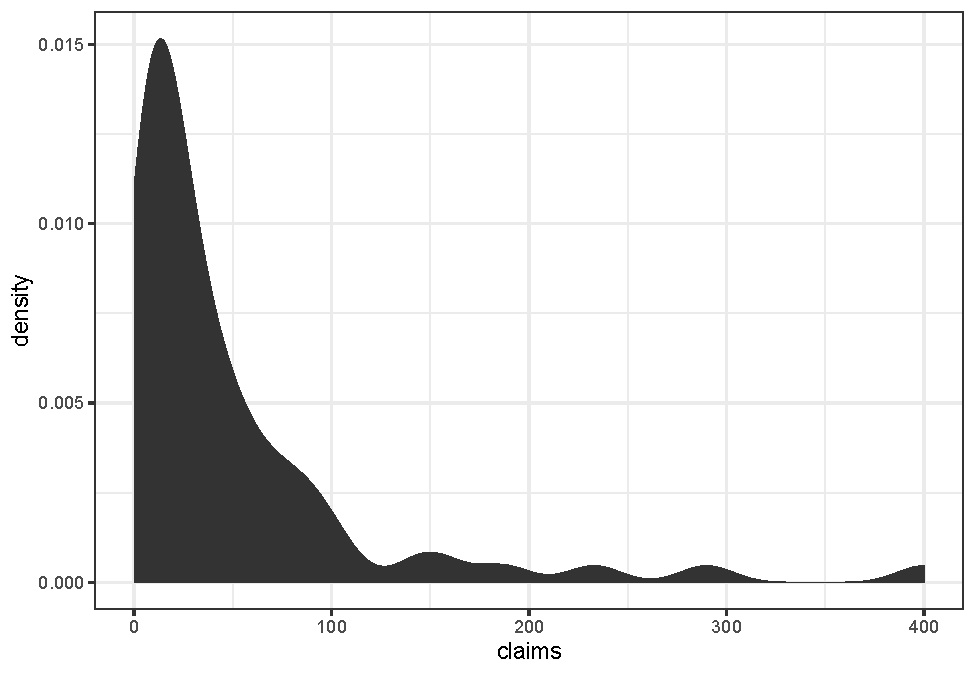
\includegraphics{04-visualization_files/figure-latex/unnamed-chunk-5-1.pdf}

\hypertarget{step-3-add-a-plot}{%
\section{Step 3: Add a plot}\label{step-3-add-a-plot}}

We add an xy plot.

\begin{Shaded}
\begin{Highlighting}[]
\NormalTok{p }\OperatorTok{+}\StringTok{ }\KeywordTok{geom_point}\NormalTok{()}
\end{Highlighting}
\end{Shaded}

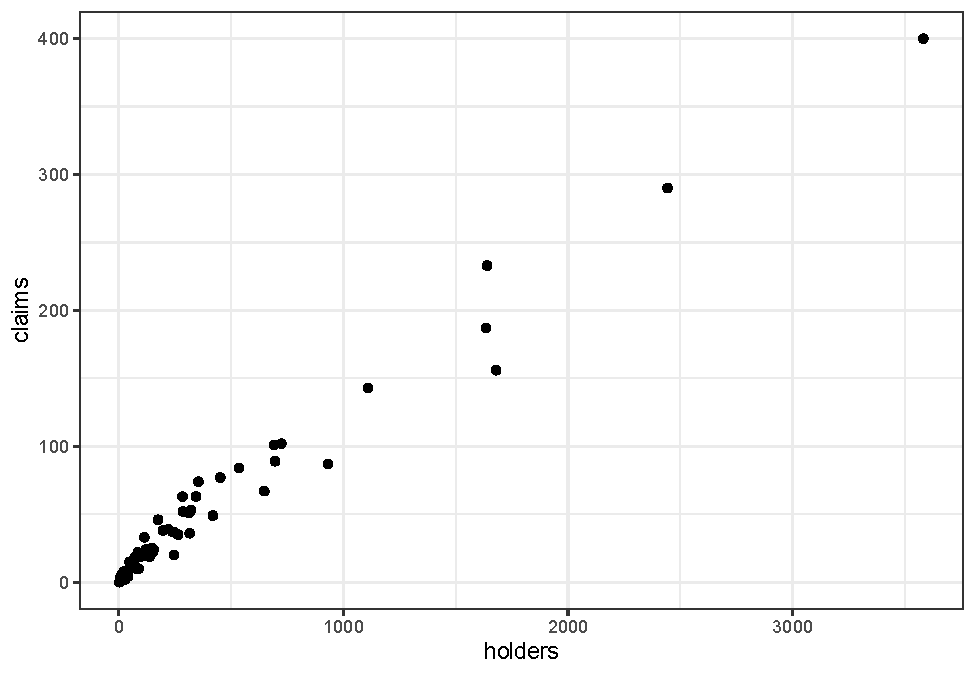
\includegraphics{04-visualization_files/figure-latex/unnamed-chunk-6-1.pdf}

We can also create a bar plot.

\begin{Shaded}
\begin{Highlighting}[]
\NormalTok{p }\OperatorTok{+}\StringTok{ }\KeywordTok{geom_bar}\NormalTok{(}\DataTypeTok{stat =} \StringTok{"identity"}\NormalTok{)}
\end{Highlighting}
\end{Shaded}

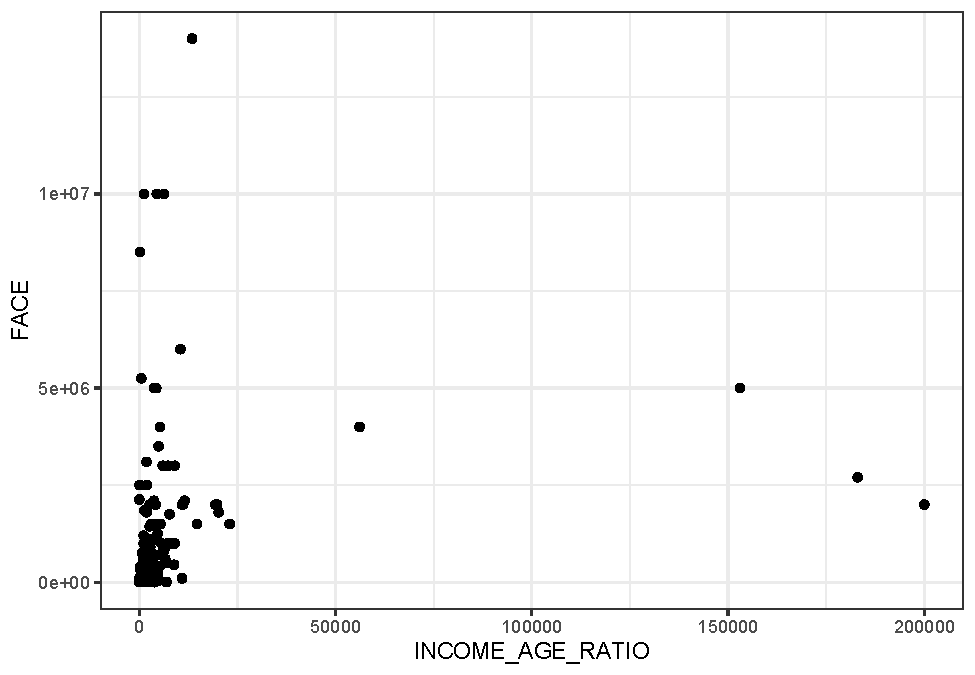
\includegraphics{04-visualization_files/figure-latex/unnamed-chunk-7-1.pdf}

Creating histograms is even easier. Just specify the column that you want to graph as the x column. No y is needed because a histogram is one-dimensional.

Take a x to be a random variable from a gamma distribution.

\begin{Shaded}
\begin{Highlighting}[]
\NormalTok{gamma =}\StringTok{ }\KeywordTok{tibble}\NormalTok{(}\DataTypeTok{x =} \KeywordTok{rgamma}\NormalTok{(}\DecValTok{1000}\NormalTok{, }\DataTypeTok{shape =} \DecValTok{1}\NormalTok{, }\DataTypeTok{rate =} \DecValTok{2}\NormalTok{))}
\end{Highlighting}
\end{Shaded}

\begin{Shaded}
\begin{Highlighting}[]
\NormalTok{p <-}\StringTok{ }\NormalTok{gamma }\OperatorTok\StringTok{ }\KeywordTok{ggplot}\NormalTok{(}\KeywordTok{aes}\NormalTok{(}\DataTypeTok{x =}\NormalTok{ x))}
\NormalTok{p }\OperatorTok{+}\StringTok{ }\KeywordTok{geom_histogram}\NormalTok{()}
\end{Highlighting}
\end{Shaded}

\begin{verbatim}
## `stat_bin()` using `bins = 30`. Pick better value with `binwidth`.
\end{verbatim}

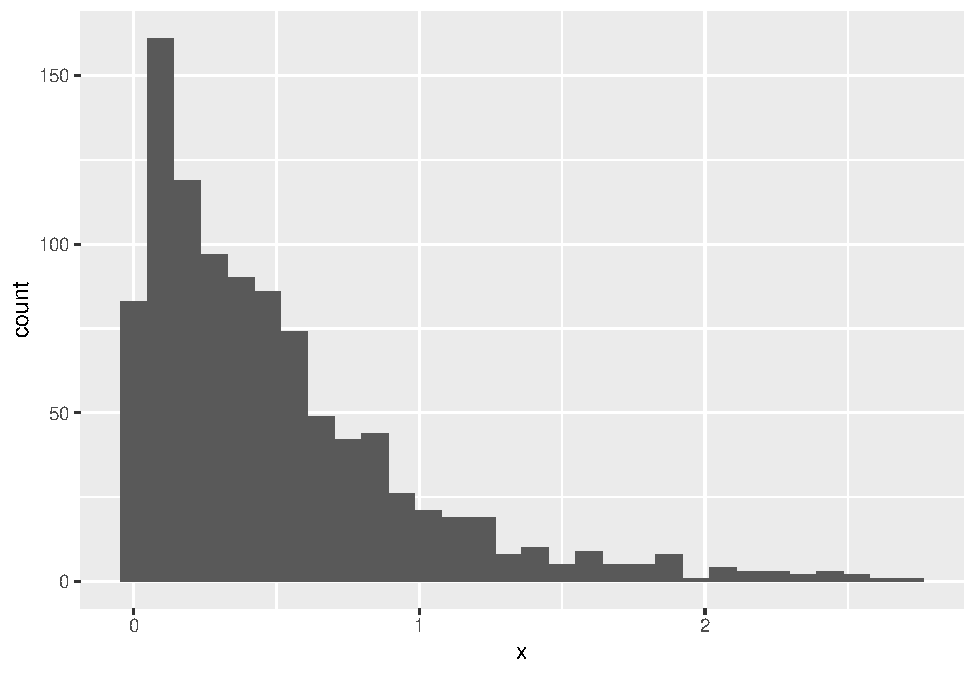
\includegraphics{04-visualization_files/figure-latex/unnamed-chunk-9-1.pdf}

We can graph a density instead of a histogram by using \texttt{geom\_density} instead of \texttt{geom\_hist}.

\begin{Shaded}
\begin{Highlighting}[]
\NormalTok{p }\OperatorTok{+}\StringTok{ }\KeywordTok{geom_density}\NormalTok{(}\DataTypeTok{fill =} \StringTok{"grey"}\NormalTok{)}
\end{Highlighting}
\end{Shaded}

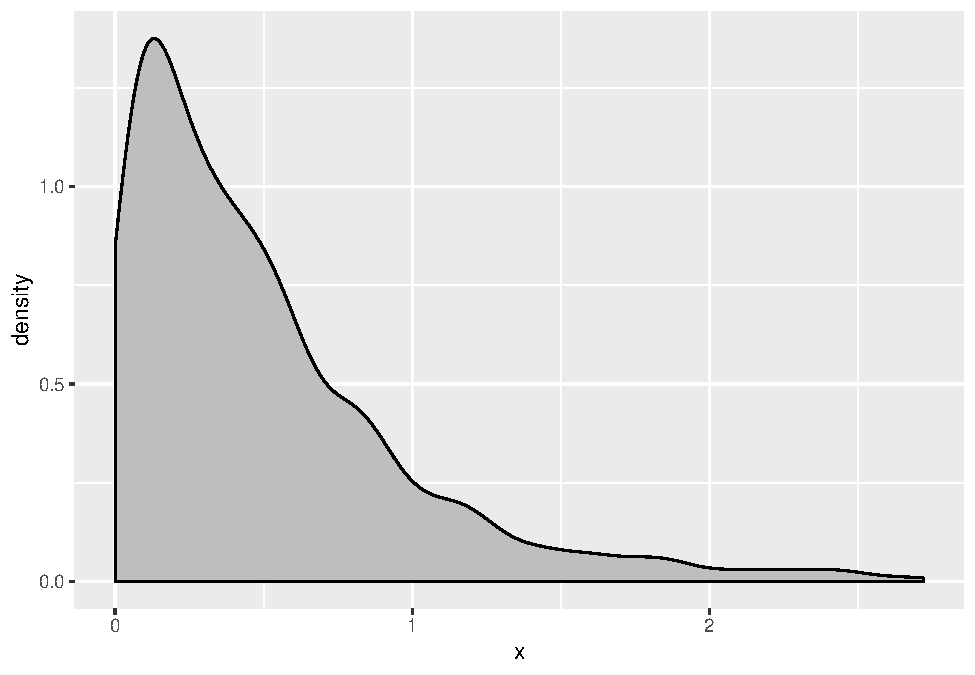
\includegraphics{04-visualization_files/figure-latex/unnamed-chunk-10-1.pdf}

\hypertarget{tree-based-models}{%
\chapter{Tree-based models}\label{tree-based-models}}

\hypertarget{decision-trees}{%
\section{Decision Trees}\label{decision-trees}}

Decision trees can be used for either classification or regression problems. The model structure is a series of yes/no questions. Depending on how each observation answers these questions, a prediction is made.

The below example shows how a single tree can predict health claims.

\begin{itemize}
\tightlist
\item
  For non-smokers, the predicted annual claims are 8,434. This represents 80\% of the observations
\item
  For smokers with a \texttt{bmi} of less than 30, the predicted annual claims are 21,000. 10\% of patients fall into this bucket.
\item
  For smokers with a \texttt{bmi} of more than 30, the prediction is 42,000. This bucket accounts for 11\% of patients.
\end{itemize}

\begin{figure}
\centering
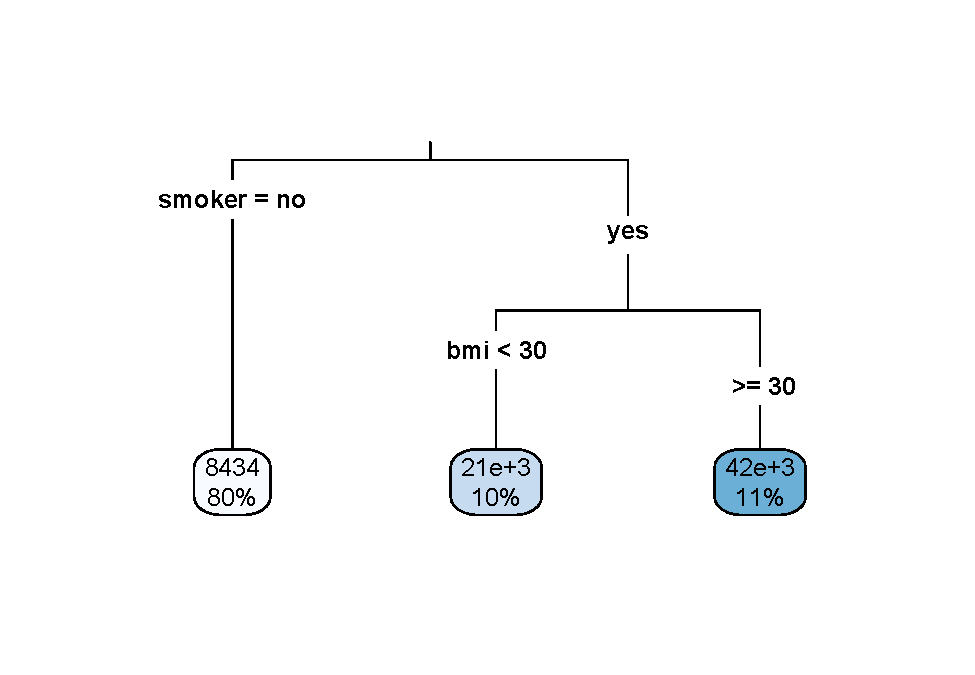
\includegraphics{06-tree-based-models_files/figure-latex/unnamed-chunk-2-1.pdf}
\caption{\label{fig:unnamed-chunk-2}Decision tree of health costs}
\end{figure}

We can cut the data set up into these groups and look at the claim costs. From this grouping, we can see that \texttt{smoker} is the most important variable as the difference in average claims is about 20,000.

\begin{longtable}[]{@{}lllr@{}}
\toprule
smoker & bmi\_30 & mean\_claims & percent\tabularnewline
\midrule
\endhead
no & bmi \textless{} 30 & \$7,977.03 & 0.38\tabularnewline
no & bmi \textgreater= 30 & \$8,842.69 & 0.42\tabularnewline
yes & bmi \textless{} 30 & \$21,363.22 & 0.10\tabularnewline
yes & bmi \textgreater= 30 & \$41,557.99 & 0.11\tabularnewline
\bottomrule
\end{longtable}

This was a very simple example because there were only two variables. If we have more variables, the tree will get large very quickly. This will result in overfitting; there will be good performance on the training data but poor performance on the test data.

The step-by-step process of building a tree is

\textbf{Step 1: Choose a variable at random.}

This could be any variable in \texttt{age}, \texttt{children}, \texttt{charges}, \texttt{sex}, \texttt{smoker}, \texttt{age\_bucket}, \texttt{bmi}, or \texttt{region}.

\textbf{Step 2: Find the split point which best seperates observations out based on the value of \(y\). A good split is one where the \(y\)'s are very different. * }

In this case, \texttt{smoker} was chosen. Then we can only split this in one way: \texttt{smoker\ =\ 1} or \texttt{smoker\ =\ 0}.

Then for each of these groups, smokers and non-smokers, choose another variable at random. In this case, for no-smokers, \texttt{age} was chosen. To find the best cut point of \texttt{age}, look at all possible age cut points from 18, 19, 20, 21, \ldots, 64 and choose the one which best separates the data.

There are three ways of deciding where to split

\begin{itemize}
\tightlist
\item
  \emph{Entropy} (aka, information gain)
\item
  \emph{Gini}
\item
  \emph{Classification error}
\end{itemize}

Of these, only the first two are commonly used. The exam is not going to ask you to calculate either of these. Just know that neither method will work better on all data sets, and so the best practice is to test both and compare the performance.

\textbf{Step 3: Continue doing this until a stopping criteria is reached. For example, the minimum number of observations is 5 or less.}

As you can see, this results in a very deep tree.

\begin{Shaded}
\begin{Highlighting}[]
\NormalTok{tree <-}\StringTok{ }\KeywordTok{rpart}\NormalTok{(}\DataTypeTok{formula =}\NormalTok{ charges }\OperatorTok{~}\StringTok{  }\NormalTok{., }\DataTypeTok{data =}\NormalTok{ health_insurance,}
              \DataTypeTok{control =} \KeywordTok{rpart.control}\NormalTok{(}\DataTypeTok{cp =} \FloatTok{0.003}\NormalTok{))}
\KeywordTok{rpart.plot}\NormalTok{(tree, }\DataTypeTok{type =} \DecValTok{3}\NormalTok{)}
\end{Highlighting}
\end{Shaded}

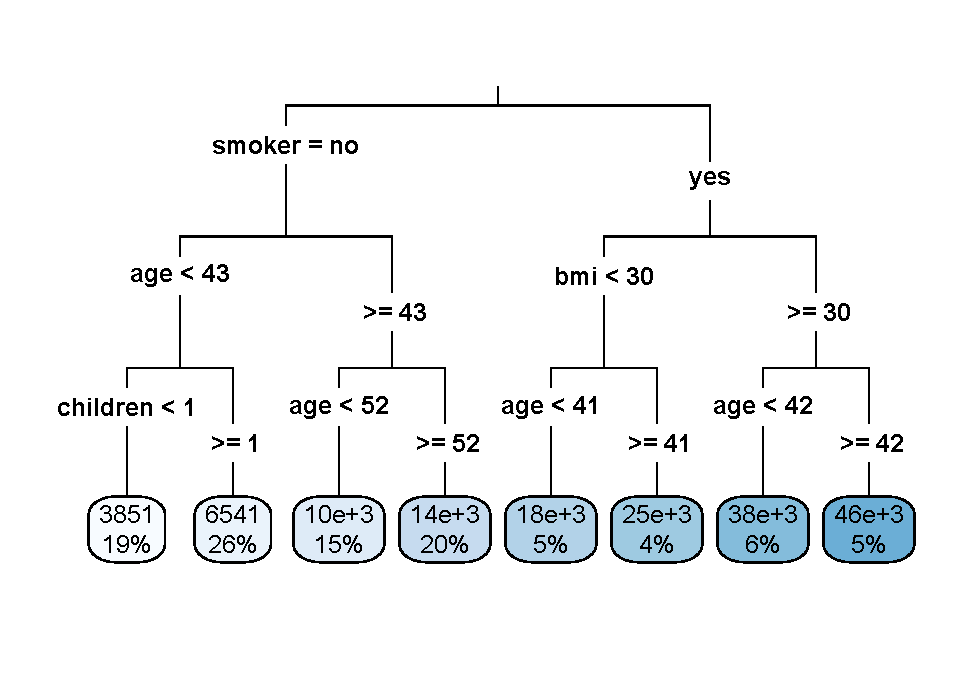
\includegraphics{06-tree-based-models_files/figure-latex/unnamed-chunk-4-1.pdf}

\textbf{Step 4: Apply cost comlexity pruning to simplify the tree}

Intuitively, we know that the above model would perform poorly due to overfitting. We want to make it simpler by removing nodes. This is very similar to how in linear models we reduce complexity by reducing the number of coefficients.

A measure of the depth of the tree is the \emph{complexity}. You can think of \(|T|\) as the ``degrees of freedom'' in a linear model. In the above example, \(|T| = 8\). The amount of penalization is controlled by \(\alpha\). This is very similar to \(\lambda\) in the Lasso.

To calculate the cost of a tree, number the terminal nodes from \(1\) to \(|T|\), and let the set of observations that fall into the \(mth\) bucket be \(R_m\). Then add up the squared error over all terminal nodes to the penalty term.

\[
\text{Cost}_\alpha(T) = \sum_{m=1}^{|T|} \sum_{R_m}(y_i - \hat{y}_{Rm})^2 + \alpha |T|
\]

\textbf{Step 5: Use cross-validation to select the best alpha}

The cost is controlled by the \texttt{CP} parameter. In the above example, did you notice the line \texttt{rpart.control(cp\ =\ 0.003)}? This is telling \texttt{rpart} to continue growing the tree until the CP reaches 0.003. At each subtree, we can measure the cost \texttt{CP} as well as the cross-validation error \texttt{xerror}.

This is stored in the \texttt{cptable}

\begin{Shaded}
\begin{Highlighting}[]
\KeywordTok{library}\NormalTok{(kableExtra)}
\KeywordTok{library}\NormalTok{(tidyverse)}
\NormalTok{tree <-}\StringTok{ }\KeywordTok{rpart}\NormalTok{(}\DataTypeTok{formula =}\NormalTok{ charges }\OperatorTok{~}\StringTok{  }\NormalTok{., }\DataTypeTok{data =}\NormalTok{ health_insurance,}
              \DataTypeTok{control =} \KeywordTok{rpart.control}\NormalTok{(}\DataTypeTok{cp =} \FloatTok{0.0001}\NormalTok{))}
\NormalTok{cost <-}\StringTok{ }\NormalTok{tree}\OperatorTok{$}\NormalTok{cptable }\OperatorTok\StringTok{ }
\StringTok{  }\KeywordTok{as_tibble}\NormalTok{() }\OperatorTok\StringTok{ }
\StringTok{  }\KeywordTok{select}\NormalTok{(nsplit, CP, xerror) }

\NormalTok{cost }\OperatorTok\StringTok{ }\KeywordTok{head}\NormalTok{()}
\end{Highlighting}
\end{Shaded}

\begin{verbatim}
## # A tibble: 6 x 3
##   nsplit      CP xerror
##    <dbl>   <dbl>  <dbl>
## 1      0 0.620    1.00 
## 2      1 0.144    0.382
## 3      2 0.0637   0.240
## 4      3 0.00967  0.179
## 5      4 0.00784  0.172
## 6      5 0.00712  0.167
\end{verbatim}

As more splits are added, the cost continues to decrease, reaches a minimum, and then begins to increase.

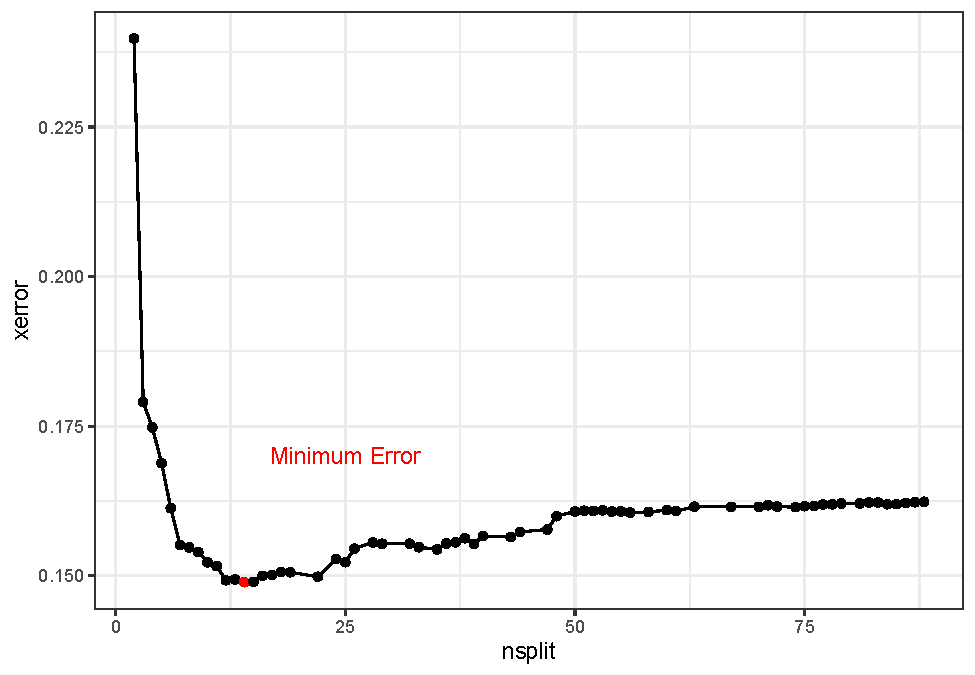
\includegraphics{06-tree-based-models_files/figure-latex/unnamed-chunk-6-1.pdf}

To optimize performance, choose the number of splits which has the lowest error. Often, though, the goal of using a decision tree is to create a simple model. In this case, we can err or the side of a lower \texttt{nsplit} so that the tree is shorter and more interpretable. All of the questions on so far have only used decision trees for interpretability, and a different model method has been used when predictive power is needed.

You will typically be given the below code, which does this automatically. To get full credit on decision tree questions, mention that you used cross-validation to select the number of splits.

\begin{Shaded}
\begin{Highlighting}[]
\NormalTok{pruned_tree <-}\StringTok{ }\KeywordTok{prune}\NormalTok{(tree,}\DataTypeTok{cp =}\NormalTok{ tree}\OperatorTok{$}\NormalTok{cptable[}\KeywordTok{which.min}\NormalTok{(tree}\OperatorTok{$}\NormalTok{cptable[, }\StringTok{"xerror"}\NormalTok{]), }\StringTok{"CP"}\NormalTok{])}
\end{Highlighting}
\end{Shaded}

\hypertarget{advantages-and-disadvantages}{%
\section{Advantages and disadvantages}\label{advantages-and-disadvantages}}

\textbf{Advantages}

\begin{itemize}
\tightlist
\item
  Easy to interpret
\item
  Captures interaction effects
\item
  Captures non-linearities
\item
  Handles continuous and categorical data
\item
  Handles missing values
\end{itemize}

\textbf{Disadvantages}

\begin{itemize}
\tightlist
\item
  Is a ``weak learner'' because of low predictive power
\item
  Does not work on small data sets
\item
  Is often a simplification of the underlying process because all observations at terminal nodes have equal predicted values
\item
  Is biased towards selecting high-cardinality features because more possible split points for these features tend to lead to overfitting
\item
  High variance (which can be alleviated with stricter parameters) leads the ``easy to interpret results'' to change upon retraining
  Unable to predict beyond the range of the training data for regression (because each predicted value is an average of training samples)
\end{itemize}

\begin{longtable}[]{@{}ll@{}}
\toprule
Readings &\tabularnewline
\midrule
\endhead
ISLR 8.1.1 Basics of Decision Trees &\tabularnewline
ISLR 8.1.2 Classification Trees &\tabularnewline
\href{https://cran.r-project.org/web/packages/rpart/vignettes/longintro.pdf}{rpart Documentation (Optional)} &\tabularnewline
\bottomrule
\end{longtable}

\hypertarget{random-forests}{%
\section{Random Forests}\label{random-forests}}

\textbf{Advantages}

\begin{itemize}
\tightlist
\item
  Resilient to overfitting due to bagging
\item
  Only one parameter to tune (mtry, the number of features considered at each split)
\item
  Very good a multi-class prediction
\item
  Nonlinearities
\item
  Interaction effects
\item
  Deal with unbalanced and missing data*Usually requires over/undersamplin
\end{itemize}

\textbf{Disadvantages}

\begin{itemize}
\tightlist
\item
  Does not work on small data sets
\item
  Weaker performance than other methods (GBM, NN)
\item
  Unable to predict beyond training data for regression
\end{itemize}

\begin{longtable}[]{@{}ll@{}}
\toprule
Readings &\tabularnewline
\midrule
\endhead
ISLR 8.1.1 Basics of Decision Trees &\tabularnewline
ISLR 8.1.2 Classification Trees &\tabularnewline
\bottomrule
\end{longtable}

\hypertarget{gradient-boosted-trees}{%
\section{Gradient Boosted Trees}\label{gradient-boosted-trees}}

\begin{itemize}
\tightlist
\item
  High prediction accuracy
\item
  Closest model to a ``silver bullet'' that exists
\item
  Nonlinearities, interaction effects, resilient to outliers, corrects for missing values
\item
  Deals with class imbalance directly through by weighting observations
\end{itemize}

\textbf{Disadvantages}

\begin{itemize}
\tightlist
\item
  Requires large sample size
\item
  Longer training time
\item
  Does not detect linear combinations of features. These must be engineered
  Can overfit if not tuned correctly
\end{itemize}

\begin{longtable}[]{@{}ll@{}}
\toprule
Readings &\tabularnewline
\midrule
\endhead
ISLR 8.1.1 Basics of Decision Trees &\tabularnewline
ISLR 8.1.2 Classification Trees &\tabularnewline
\bottomrule
\end{longtable}

\hypertarget{a-mini-exam-example}{%
\chapter{A Mini-Exam Example}\label{a-mini-exam-example}}

A common regret of students who failed exam PA is that they did not start doing practice exams soon enough. Here is a simple practice exam to help you to understand what concepts that you should focus on learning, to become familiar with the format, and to test your technical skills with R, RStudio, and MS Word.

\hypertarget{project-statement}{%
\section{Project Statement}\label{project-statement}}

ABC Health Insurance company is building a model to predict medical claims. Using only \texttt{age} and \texttt{sex} information from the prior year, build a model to predict claims for the next year.

\hypertarget{describe-the-data-1-point}{%
\subsection{Describe the data (1 point)}\label{describe-the-data-1-point}}

\begin{Shaded}
\begin{Highlighting}[]
\KeywordTok{library}\NormalTok{(tidyverse)}
\NormalTok{data <-}\StringTok{ }\KeywordTok{read_csv}\NormalTok{(}\StringTok{"C:/Users/sam.castillo/Desktop/R Manual Data/health_insurance.csv"}\NormalTok{) }\OperatorTok\StringTok{ }
\StringTok{  }\KeywordTok{select}\NormalTok{(age, sex, charges) }\OperatorTok\StringTok{  }\CommentTok{#put this into an r library}
\StringTok{  }\KeywordTok{rename}\NormalTok{(}\DataTypeTok{claims =}\NormalTok{ charges)}

\NormalTok{data }\OperatorTok\StringTok{ }\KeywordTok{summary}\NormalTok{()}
\end{Highlighting}
\end{Shaded}

\begin{verbatim}
##       age            sex                claims     
##  Min.   :18.00   Length:1338        Min.   : 1122  
##  1st Qu.:27.00   Class :character   1st Qu.: 4740  
##  Median :39.00   Mode  :character   Median : 9382  
##  Mean   :39.21                      Mean   :13270  
##  3rd Qu.:51.00                      3rd Qu.:16640  
##  Max.   :64.00                      Max.   :63770
\end{verbatim}

\begin{Shaded}
\begin{Highlighting}[]
\NormalTok{data }\OperatorTok\StringTok{ }\KeywordTok{dim}\NormalTok{()}
\end{Highlighting}
\end{Shaded}

\begin{verbatim}
## [1] 1338    3
\end{verbatim}

\begin{quote}
The data consists of 1,338 policies with age and sex information. The objective is to predict future claims.
\end{quote}

\hypertarget{create-a-histogram-of-the-claims-and-comment-on-the-shape-1-point}{%
\subsection{Create a histogram of the claims and comment on the shape (1 point)}\label{create-a-histogram-of-the-claims-and-comment-on-the-shape-1-point}}

The distribution of claims is strictly positive and right skewed.

\begin{Shaded}
\begin{Highlighting}[]
\NormalTok{data }\OperatorTok\StringTok{ }\KeywordTok{ggplot}\NormalTok{(}\KeywordTok{aes}\NormalTok{(claims)) }\OperatorTok{+}\StringTok{ }\KeywordTok{geom_histogram}\NormalTok{()}
\end{Highlighting}
\end{Shaded}

\begin{verbatim}
## `stat_bin()` using `bins = 30`. Pick better value with `binwidth`.
\end{verbatim}

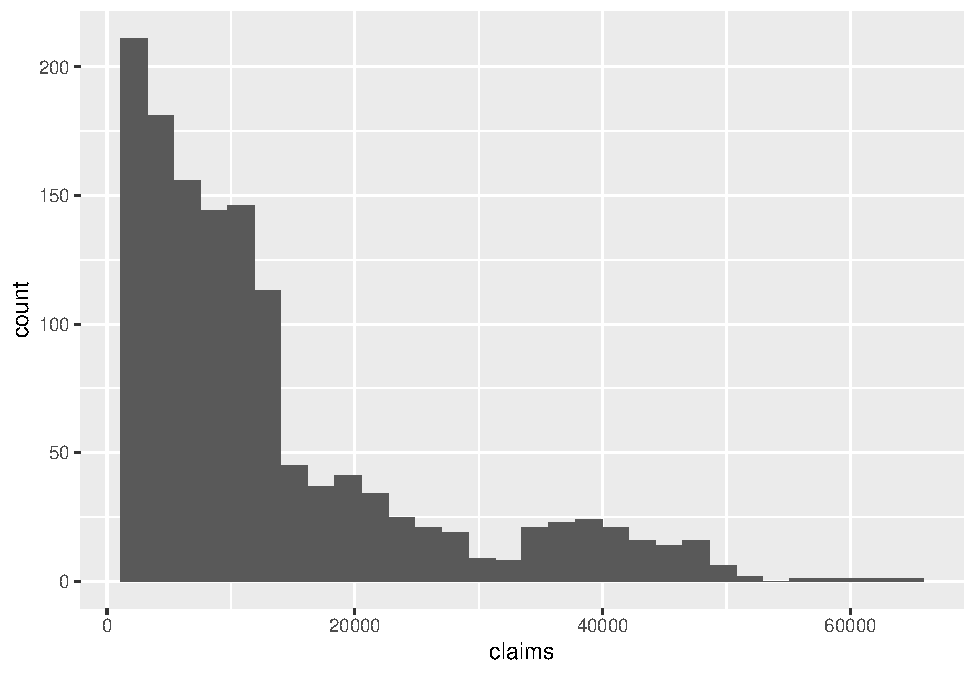
\includegraphics{07-example_files/figure-latex/unnamed-chunk-2-1.pdf}

\hypertarget{fit-a-linear-model-1-point}{%
\subsection{Fit a linear model (1 point)}\label{fit-a-linear-model-1-point}}

\begin{Shaded}
\begin{Highlighting}[]
\NormalTok{model =}\StringTok{ }\KeywordTok{lm}\NormalTok{(claims }\OperatorTok{~}\StringTok{ }\NormalTok{age }\OperatorTok{+}\StringTok{ }\NormalTok{sex, }\DataTypeTok{data =}\NormalTok{ data)}
\end{Highlighting}
\end{Shaded}

\hypertarget{describe-the-relationship-between-age-sex-and-claim-costs-1-point}{%
\subsection{Describe the relationship between age, sex, and claim costs (1 point)}\label{describe-the-relationship-between-age-sex-and-claim-costs-1-point}}

\begin{quote}
We fit a linear model to the claim costs using age and sex as predictor variables. The coefficient of \texttt{age} is 258, indicating that the claim costs increase by \$258 for every one-unit increase in the policyholder's age. The cofficient of 1538 on \texttt{sexmale} indicates that on average, men have \$1538 higher claims than women do.
\end{quote}

\begin{Shaded}
\begin{Highlighting}[]
\KeywordTok{coefficients}\NormalTok{(model)}
\end{Highlighting}
\end{Shaded}

\begin{verbatim}
## (Intercept)         age     sexmale 
##   2343.6249    258.8651   1538.8314
\end{verbatim}

\hypertarget{write-a-summary-of-steps-1-4-in-non-technical-language-1-point}{%
\subsection{Write a summary of steps 1-4 in non-technical language (1 point)}\label{write-a-summary-of-steps-1-4-in-non-technical-language-1-point}}

\begin{quote}
ABC Health is interested in predicting the future claims for a group of policyholders. We began by collecting data on 1,538 policy holders which recorded their age, sex, and annual claims. We then created a histogram of the claim costs. A linear model which shows that claim costs increase as age increases, and are higher for men on average.
\end{quote}

\hypertarget{practice-exam}{%
\chapter{Practice Exam}\label{practice-exam}}

This is a practice exam that is based on the December 2018 PA exam. This is easier than the actual exam.

\hypertarget{prior-exams}{%
\chapter{Prior Exams}\label{prior-exams}}

There are the exams and solutions published by the SOA.

\bibliography{book.bib,packages.bib}


\end{document}
